\chapter{МЕТОДЫ УПРАВЛЕНИЯ ЭЛЕКТРОПНЕВМАТИЧЕСКИМ ПРИВОДОМ С ДИСКРЕТНЫМ УПРАВЛЕНИЕМ}\label{ch:ch3}
Управление электропневматическими приводами с дискретными распределителями представляет
собой комплексную задачу, обусловленную нелинейной динамикой пневматических систем и
дискретным характером управляющих воздействий. Эффективное решение данной задачи требует
применения специализированных алгоритмов, способных обеспечить высокую точность позиционирования и
быстродействие системы при ограниченном наборе управляющих состояний. Особый интерес представляет адаптация
классических методов управления к специфике дискретных пневматических систем.

В рамках настоящего исследования рассматривается широкий спектр подходов к управлению электропневматическими
приводами, включающий как модифицированные класические алгоритмы, так и современные адаптивные методы.
Исследуются применение широтно-импульсной модуляции (ШИМ)
в сочетании с классическими регуляторами, такими как ПИД-регулятор и его модификации,
скользящее управление, нечеткое управление, прогнозное управление.
Выбор данных методов обусловлен необходимостью комплексного анализа возможностей оптимизации управления
с учетом специфики дискретных пневматических систем. Каждый из рассматриваемых подходов обладает
уникальными преимуществами и ограничениями, детальное изучение которых позволит сформировать
всестороннее представление о перспективах совершенствования алгоритмов управления
электропневматическими приводами с дискретными распределителями.


% 
\section{Анализ режимов работы электропневмопривода}\label{sec:ch3/sec1}

Функционирование электропневмопривода с дискретными распределителями характеризуется конечным
множеством возможных состояний системы, определяемых комбинациями состояний распределителей.
Математически пространство состояний распределителей может быть представлено как:

\begin{equation}\label{eq:state_space}
	\mathbf{U} = \left\{
	[u_1, u_2, u_3, u_4] | u_i \in {0,1}, i = 1,\dots,4
	\right\},
\end{equation}
где $u_i$ -- состояние i-го распределителя (0 - закрыт, 1 - открыт).

Теоретически система, как описано ранее, допускает $2^4 = 16$ различных комбинаций состояний распределителей.
Однако с учетом физических ограничений и требований безопасности целесообразно использование только определенного
подмножества состояний, формирующих основные режимы работы привода.

Классификация этих режимов представлена в следующей таблице \ref{tab:operation_modes}.

\begin{table}[htbp]
	\centering
	\caption{Режимы работы электропневматического привода с дискретными распределителями}
	\label{tab:operation_modes}
	\small
	\begin{tabular}{lcll}
		\midrule
		\textbf{Режим}           & $[u_1,u_2,u_3,u_4]$ & \textbf{Движение} & \textbf{Динамика} \\
		\midrule
		СиП\textsuperscript{1}   & $[1,0,0,1]$         &
		Макс. положит. ускорение &
		$M\ddot{x} = p_\text{п}F_1 - p_\text{атм}F_2 - R_\text{тр}$                            \\

		СрП\textsuperscript{2}   & $[1,0,0,0]$         &
		Умер. положит. ускорение &
		$M\ddot{x} = p_\text{п}F_1 - p_2F_2 - R_\text{тр}$                                     \\

		СлП\textsuperscript{3}   & $[0,0,0,1]$         &
		Мин. положит. ускорение  &
		$M\ddot{x} = p_1F_1 - p_\text{атм}F_2 - R_\text{тр}$                                   \\

		СиО.\textsuperscript{4}  & $[0,1,1,0]$         &
		Макс. отриц. ускорение   &
		$M\ddot{x} = p_\text{атм}F_1 - p_\text{п}F_2 - R_\text{тр}$                            \\

		СрО\textsuperscript{5}   & $[0,0,1,0]$         &
		Умер. отриц. ускорение   &
		$M\ddot{x} = p_1F_1 - p_\text{п}F_2 - R_\text{тр}$                                     \\

		СлО\textsuperscript{6}   & $[0,1,0,0]$         &
		Мин. отриц. ускорение    &
		$M\ddot{x} = p_\text{атм}F_1 - p_2F_2 - R_\text{тр}$                                   \\

		\hline
		Н                        & $[0,0,0,0]$         &
		Фиксация положения       &
		$M\ddot{x} = p_1F_1 - p_2F_2 - R_\text{тр}$                                            \\
		\midrule
	\end{tabular}
	\begin{tablenotes}
		\scriptsize
		\item[1] СиП -- сильное положительное ускорение
		\item[2] СрП -- среднее положительное ускорение
		\item[3] СлП -- слабое положительное ускорение
		\item[4] СлО -- сильное отрицательное ускорение
		\item[5] СрО -- среднее отрицательное ускорение
		\item[6] СлО -- слабое отрицательное ускорение
		\item[7] Н -- удержание
	\end{tablenotes}
\end{table}

Динамическое поведение электропневматического привода для каждого режима может быть
проанализировано как в пространстве давлений, так и в фазовом пространстве
скорость-положение. Векторное поле в фазовом пространстве описывается системой дифференциальных уравнений:

\begin{equation}
	\begin{cases}
		\dot{x} = v \\
		\dot{v} = \frac{1}{M}(p_1F_1 - p_2F_2 - R_\text{тр}(v))
	\end{cases}
\end{equation}
где $(x,v)$ -- координаты точки в фазовом пространстве.

Для комплексного понимания динамических процессов в пневмоприводе целесообразно рассмотреть
сравнительные характеристики изменения давлений в полостях пневмоцилиндра
при различных режимах работы, представленные на рисунке \ref{fig:pressure_comparison}.
На графиках отображены процессы для положительного перемещения (выдвижения штока),
поскольку для отрицательного перемещения (втягивания штока) динамика является аналогичной с учетом симметрии системы.

\begin{figure}[htbp]
	\centering
	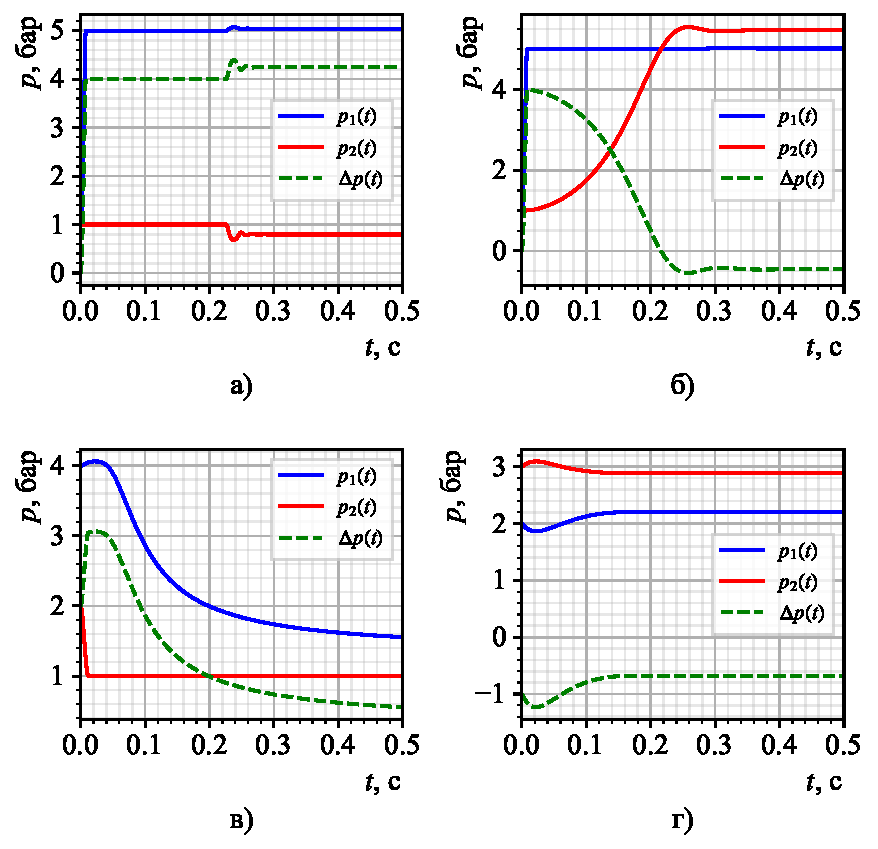
\includegraphics{part3/pressure_dynamics.pdf}
	\caption{Сравнение динамики установления давлений в различных режимах работы:\\
		а) сильное ускорение; б) умеренное ускорение; в) слабое ускорение; г) режим удержания}
	\label{fig:pressure_comparison}
\end{figure}

Представленные характеристик показывает существенное различие в динамике установления давлений для разных режимов работы.

В режиме сильного положительного ускорения [1,0,0,1] наблюдается максимальный
перепад давлений между полостями цилиндра, что подтверждается системой уравнений:

$$\begin{cases}
		\dot{p}_1 = \frac{\gamma RT_1}{V_1(x)}(G_{1,max} - \frac{p_1}{RT_1}F_1\dot{x}) \\
		\dot{p}_2 = \frac{\gamma RT_2}{V_2(x)}(-G_{4,max} + \frac{p_2}{RT_2}F_2\dot{x})
	\end{cases}$$
где $G_{1,max}$ и $G_{4,max}$ -- максимальные массовые расходы через соответствующие распределители.

Характерной особенностью данного режима является быстрый рост давления $p_1$ до величины, близкой к давлению питания
$p_\text{п}$, с одновременным падением давления $p_2$ до атмосферного давления $p_\text{атм}$. Это обеспечивает интенсивный
разгон штока с последующим выходом на установившуюся скорость, что наглядно демонстрируется на
фазовом портрете (рис. \ref{fig:pp_strong_accelration}). Анализ фазового портрета показывает,
что процесс выхода на установившуюся скорость характеризуется движением изображающей
точки по траектории, асимптотически стремящейся к прямой $v = v_\text{уст}$.

\begin{figure}[htbp]
	\centerfloat{
		\hfill
		\subcaptionbox[List-of-Figures entry]{\label{fig:pp_strong_acceleration_positive}}{
			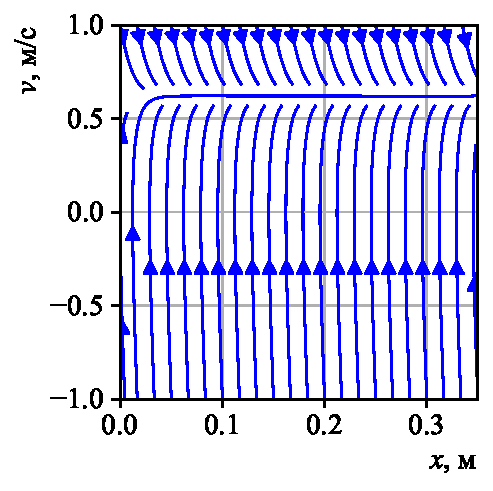
\includegraphics{part3/pp_strong_acceleration_positive.pdf} }
		\hfill
		\subcaptionbox{\label{fig:pp_strong_acceleration_negative}}{
			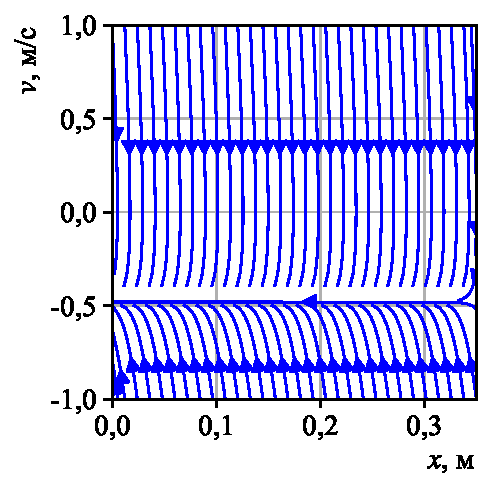
\includegraphics{part3/pp_strong_acceleration_negative.pdf} }
	}
	\caption{Фазовые портреты для режима сильного ускорения:\\
		а) положительное ускорение; б) отрицательное ускорение}
	\label{fig:pp_strong_accelration}
\end{figure}

В режимах умеренного ускорения [1,0,0,0]
наблюдается более сложная динамика, обусловленная асимметричным изменением давлений.
При данном режиме динамика давлений описывается системой:

\begin{equation}
	\begin{cases}
		\dot{p}_1 = \frac{\gamma RT_1}{V_1(x)}(G_{1,max} - \frac{p_1}{RT_1}F_1\dot{x}) \\
		\dot{p}_2 = -\frac{\gamma p_2}{V_2(x)}F_2\dot{x}
	\end{cases}
\end{equation}

Особенность данного режима заключается в том, что давление в штоковой полости изменяется согласно политропному процессу:

\begin{equation}
	p_2V_2(x)^n = p_{2,0}V_{2,0}^n = \text{const}
\end{equation}
где $p_{2,0}$ и $V_{2,0}$ -- начальное давление и объем штоковой полости соответственно в момент запирания полости;
$n$ - показатель политропы.

На фазовых портретах представленных на рисунке \ref{fig:pp_moderate_position_1} и рисунке \ref{fig:pp_moderate_position_2}
отчетливо видно влияние начальных условий на динамику системы. При большем начальном положении штока ($x_0$ равное 0,2~\si{\metre}) наблюдается более
интенсивное торможение вследствие меньшего начального объема запертой полости и, соответственно, более быстрого роста давления при сжатии воздуха.

\begin{figure}[htbp]
	\centerfloat{
		\hfill
		\subcaptionbox[List-of-Figures entry]{\label{fig:pp_medium_acceleration_x_01}}{
			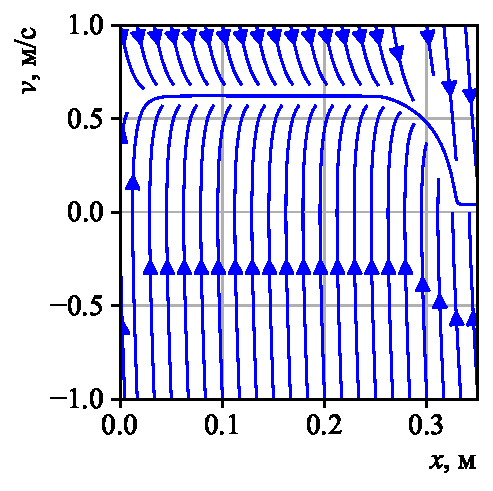
\includegraphics{part3/pp_medium_acceleration_x_01.pdf} }
		\hfill
		\subcaptionbox{\label{fig:pp_medium_acceleration_x_01_scheme}}{
			\raisebox{0.5\height}{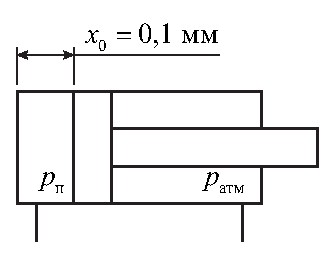
\includegraphics{part3/pp_medium_acceleration_x_01_scheme.eps}} }
	}
	\caption{Фазовый портрет и схема пневмоцилиндра при начальном положении штока $x_0 = \num{0.1}$ м ($p_{2,0} = p_\text{атм}$):\\
		а) фазовый портрет; б) схема пневмоцилиндра}
	\label{fig:pp_moderate_position_1}
\end{figure}

\begin{figure}[htbp]
	\centerfloat{
		\hfill
		\subcaptionbox[List-of-Figures entry]{\label{fig:pp_medium_acceleration_x_02}}{
			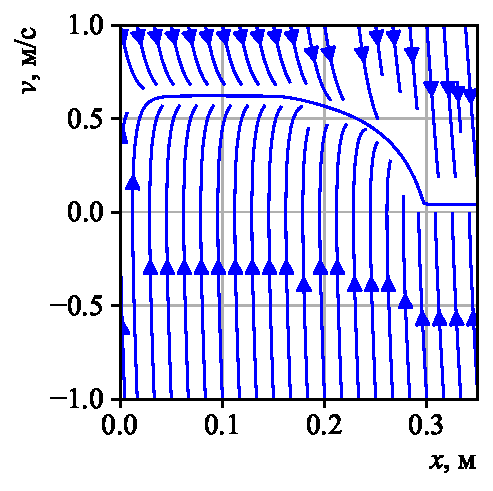
\includegraphics{part3/pp_medium_acceleration_x_02.pdf} }
		\hfill
		\subcaptionbox{\label{fig:pp_medium_acceleration_x_02_scheme}}{
			\raisebox{0.5\height}{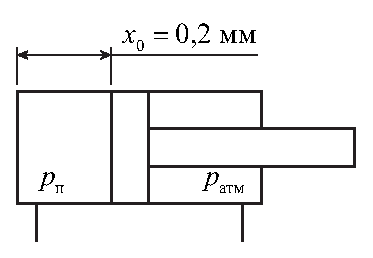
\includegraphics{part3/pp_medium_acceleration_x_02_scheme.eps}} }
	}
	\caption{Фазовый портрет и схема пневмоцилиндра при начальном положении штока $x_0 = \num{0.2}$ м ($p_{2,0} = p_\text{атм}$):\\
		а) фазовый портрет; б) схема пневмоцилиндра}
	\label{fig:pp_moderate_position_2}
\end{figure}

Для более полного понимания влияния начальных условий на динамику системы рассмотрена серия фазовых
портретов при различных комбинациях начального положения штока и давления в запираемой
полости (рис. \ref{fig:pp_moderate_matrix}). Анализ данных портретов демонстрирует, что при
фиксированном начальном положении увеличение давления $p_{2,0}$ приводит к снижению установившейся скорости
движения и увеличению интенсивности торможения. При фиксированном начальном давлении
увеличение координаты $x_0$ вызывает сокращение области достижимых состояний и смещение точки остановки к начальному положению.

\begin{figure}[htbp]
	\centerfloat{
		\hfill
		\subcaptionbox[List-of-Figures entry]{\label{fig:pp_medium_acceleration_x_01_p_2}}{
			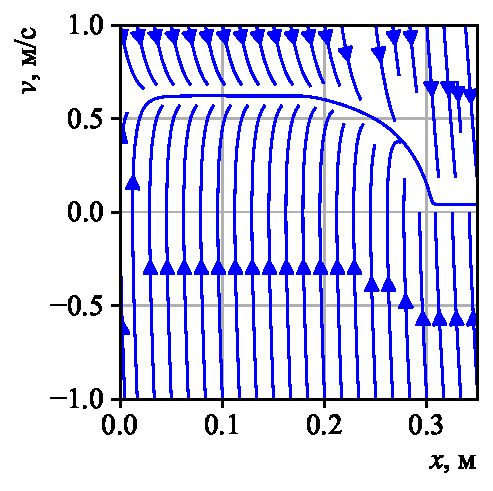
\includegraphics{part3/pp_medium_acceleration_x_01_p_2.pdf} }
		\hfill
		\subcaptionbox{\label{fig:pp_medium_acceleration_x_01_p_4}}{
			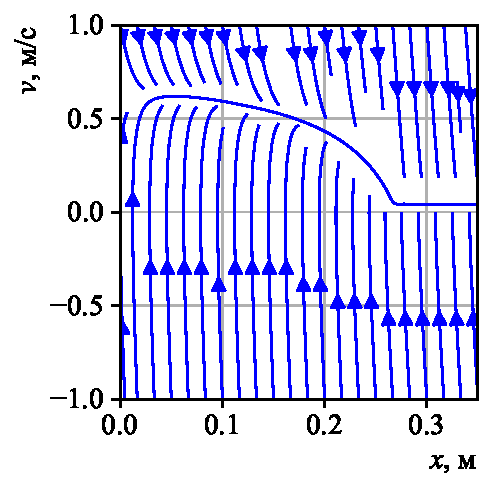
\includegraphics{part3/pp_medium_acceleration_x_01_p_4.pdf}}
		\hfill
		\subcaptionbox{\label{fig:pp_medium_acceleration_x_02_p_2}}{
			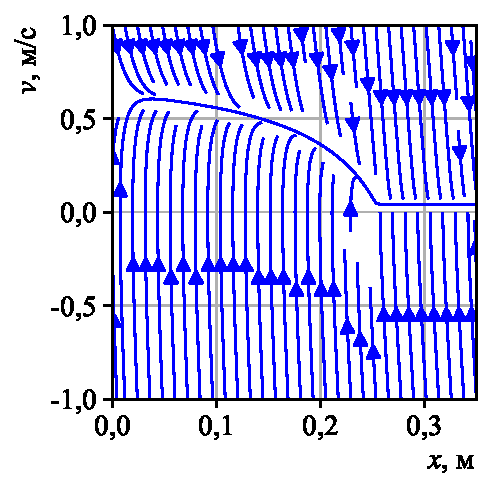
\includegraphics{part3/pp_medium_acceleration_x_02_p_2.pdf}}
		\hfill
		\subcaptionbox{\label{fig:pp_medium_acceleration_x_02_p_3}}{
			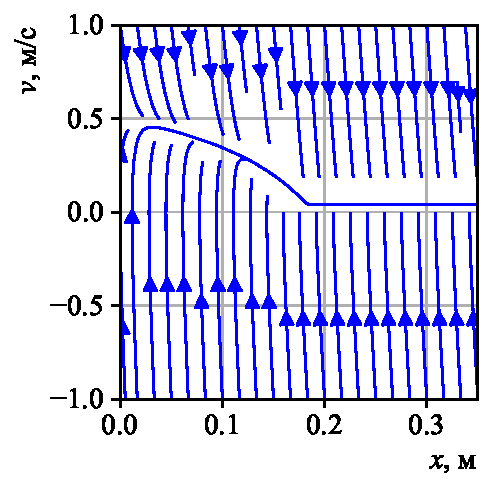
\includegraphics{part3/pp_medium_acceleration_x_02_p_4.pdf}}
	}
	\caption{Фазовые портреты при различных начальных условиях: \\
		а) $x_0 = \num{0,1}$ м, $p_{2,0} = 2$ бар; б) $x_0 = \num{0.1}$ м, $p_{2,0} = 4$ бар; \\
		в) $x_0 = \num{0.2}$ м, $p_{2,0} = 2$ бар; г) $x_0 = \num{0.2}$ м, $p_{2,0} = 4$ бар;
	}
	\label{fig:pp_moderate_matrix}
\end{figure}

Математически наблюдаемые эффекты описываются уравнением баланса сил:

\begin{equation}
	p_\text{п}F_1 - p_{2,0}\left(\frac{V_{2,0}}{V_2(x)}\right)^nF_2 = R_\text{тр}(v),
\end{equation}
где $V_2(x) = V_{2,0} + A_2(L - x)$ -- текущий объем запертой полости.

Режимы слабого ускорения [0,0,0,1] или [0,1,0,0] характеризуются минимальным перепадом давлений между
полостями пневмоцилиндра. Рассмотрим режим слабого положительного ускорения [0,0,0,1], при котором поршневая полость
изолирована, а штоковая соединена с атмосферой. Динамика давлений в данном режиме описывается системой уравнений:

$$\begin{cases}
		\dot{p}_1 = -\frac{\gamma p_1}{V_1(x)}F_1\dot{x} \\
		\dot{p}_2 = \frac{\gamma RT_2}{V_2(x)}(-G_{4,max} + \frac{p_2}{RT_2}F_2\dot{x})
	\end{cases}$$

На графиках отображенных на рисунке \ref{fig:pressure_comparison} видно, что давление $p_2$ снижается до
тмосферного значения существенно медленнее, чем в режиме сильного ускорения, в то время как
давление $p_1$ изменяется только за счет изменения объема поршневой полости. Данный процесс
характеризуется политропным изменением состояния воздуха в запертой полости:

\begin{equation}
	p_1V_1(x)^n = p_{1,0}V_{1,0}^n = \text{const}
\end{equation}
где $p_{1,0}$ и $V_{1,0}$ -- начальные значения давления и объема поршневой полости соответственно.

\begin{figure}[htbp]
	\centerfloat{
		\hfill
		\subcaptionbox[List-of-Figures entry]{\label{fig:pp_weak_acceleration_x01}}{
			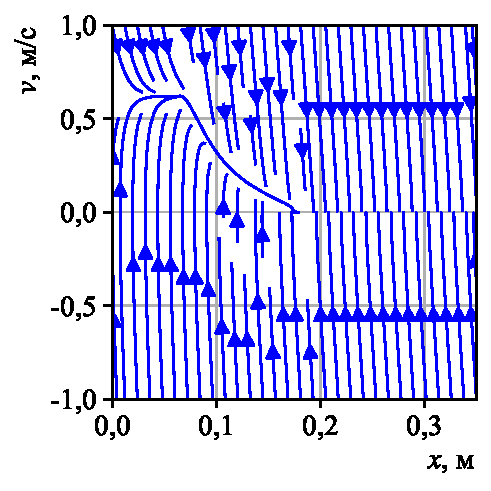
\includegraphics{part3/pp_slow_acceleration_x_01_p_3.pdf} }
		\hfill
		\subcaptionbox{\label{fig:pp_weak_acceleration_x02}}{
			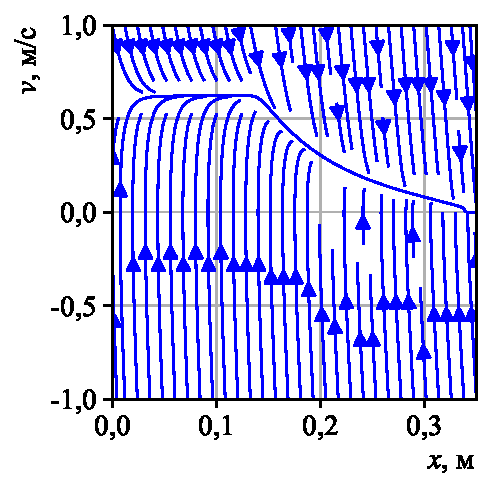
\includegraphics{part3/pp_slow_acceleration_x_02_p_3.pdf} }
	}
	\caption{Фазовые портреты для режима слабого ускорения при различных начальных условиях:\\
		а) $x_0 = \num{0.1}$ м, $p_{1,0} = 3$ бар; б) $x_0 = \num{0.2}$ м, $p_{1,0} = 3$ бар}
	\label{fig:pp_weak_acceleration}
\end{figure}

Анализ фазовых портретов представленных на рисунке \ref{fig:pp_weak_acceleration} показывает существенное влияние начального
положения штока на динамику системы. При увеличении начальной координаты $x_0$ наблюдается снижение максимально достижимой
скорости и уменьшение пути перемещения до точки остановки. Это объясняется более быстрым падением давления $p_1$ при расширении
воздуха в запертой полости большего начального объема.

Уравнение баланса сил для данного режима имеет вид:

\begin{equation}
	p_{1,0}\left(\frac{V_{1,0}}{V_1(x)}\right)^nF_1 - p_\text{атм}F_2 = R_\text{тр}(v)
\end{equation}

где $V_1(x) = V_{1,0} + A_1x$ - текущий объем поршневой полости.

Характерной особенностью режима слабого ускорения является существенная зависимость динамики
от сил трения. На фазовых портретах это проявляется в виде более крутых траекторий
торможения и меньшей области достижимых состояний по сравнению с режимами сильного и
умеренного ускорения. Данный эффект объясняется тем, что движущая сила, определяемая
разностью давлений в полостях, сопоставима по величине с силами трения.

Для оценки влияния начального давления в запертой полости на динамику системы рассмотрим
серию фазовых портретов при различных значениях $p_{1,0}$ приведенных на рисунке \ref{fig:pp_weak_pressure_matrix}.

\begin{figure}[htbp]
	\centerfloat{
		\hfill
		\subcaptionbox[List-of-Figures entry]{\label{fig:pp_weak_p2}}{
			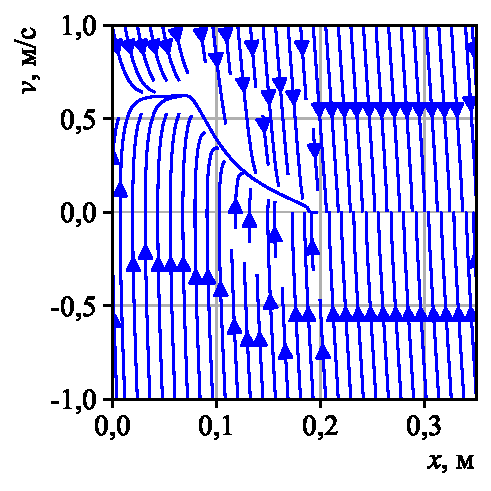
\includegraphics{part3/pp_slow_acceleration_x_015_p_2.pdf} }
		\hfill
		\subcaptionbox{\label{fig:pp_weak_p3}}{
			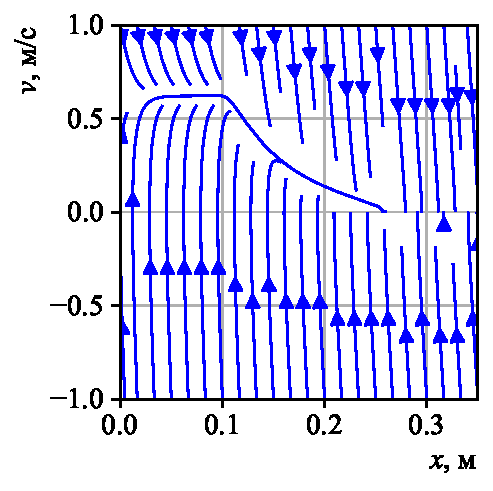
\includegraphics{part3/pp_slow_acceleration_x_015_p_3.pdf} }
		\vfill
		\subcaptionbox{\label{fig:pp_weak_p4}}{
			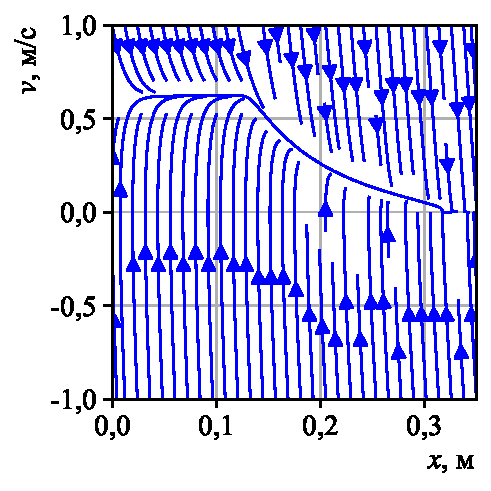
\includegraphics{part3/pp_slow_acceleration_x_015_p_4.pdf} }
	}
	\caption{Фазовые портреты при $x_0 = \num{0.15}$ м и различных начальных давлениях:\\
		а) $p_{1,0} = 2$ бар; б) $p_{1,0} = 3$ бар; в) $p_{1,0} = 4$ бар}
	\label{fig:pp_weak_pressure_matrix}
\end{figure}

Анализ представленных фазовых портретов демонстрирует, что увеличение начального давления $p_{1,0}$ приводит
к возрастанию максимальной скорости движения и увеличению дальности перемещения штока. При этом форма
фазовых траекторий становится более пологой, что свидетельствует о меньшем влиянии сил трения
на динамику системы. Данный эффект объясняется увеличением движущей силы при сохранении характера
её изменения в процессе движения.

%%%%%%%%%%%%%%%%%%%%%%%% mode 0

Режим удержания [0,0,0,0] представляет особый интерес с точки зрения
динамики электропневматического привода, поскольку в данном режиме обе полости
пневмоцилиндра оказываются изолированными.Изменение давлений при этом
происходит исключительно за счет изменения объемов полостей и описывается системой уравнений:

$$\begin{cases}
		\dot{p}_1 = -\frac{\gamma p_1}{V_1(x)}F_1\dot{x} \\
		\dot{p}_2 = -\frac{\gamma p_2}{V_2(x)}F_2\dot{x}
	\end{cases}$$

На графиках изменения давлений, согласно рисунку \ref{fig:pressure_comparison}, наблюдается характерное
политропное изменение состояния воздуха в обеих полостях, описываемое уравнениями:

\begin{equation}
	\begin{cases}
		p_1V_1(x)^n = p_{1,0}V_{1,0}^n = \text{const} \\
		p_2V_2(x)^n = p_{2,0}V_{2,0}^n = \text{const}
	\end{cases}
\end{equation}

где $p_{1,0}$, $V_{1,0}$ и $p_{2,0}$, $V_{2,0}$ -- начальные значения давлений и объемов поршневой и штоковой полостей соответственно.

Стабилизация положения штока в режиме удержания обеспечивается преимущественно силами трения, а также дополнительно
поддерживается пневматической жёсткостью, создаваемой сжатым воздухом в изолированных полостях. Баланс сил в данном режиме описывается уравнением:

\begin{equation}
	p_1F_1 - p_2F_2 = R_\text{тр}(v)
\end{equation}

\begin{figure}[htbp]
	\centerfloat{
		\hfill
		\subcaptionbox[List-of-Figures entry]{\label{fig:pp_hold_low_pressure}}{
			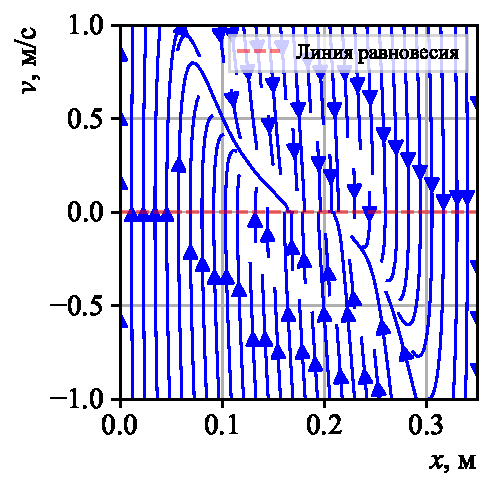
\includegraphics{part3/pp_hold_low_pressure.pdf} }
		\hfill
		\subcaptionbox{\label{fig:pp_hold_high_pressure}}{
			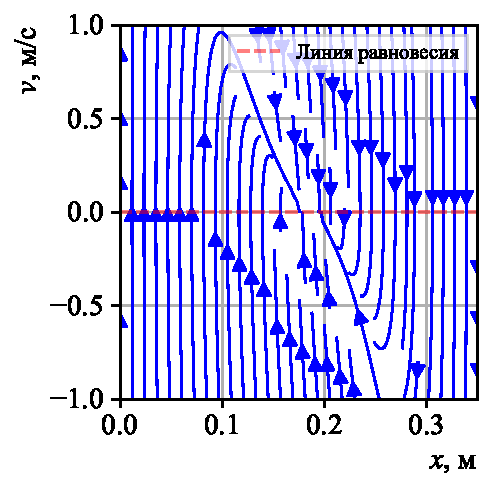
\includegraphics{part3/pp_hold_high_pressure.pdf} }
	}
	\caption{Фазовые портреты для режима удержания при различных начальных давлениях:\\
		а) низкие начальные давления ($p_{1,0} = 2$ бар, $p_{2,0} = \num{2}$ бар);\\
		б) высокие начальные давления ($p_{1,0} = 4$ бар, $p_{2,0} = \num{4}$ бар)}
	\label{fig:pp_hold_mode}
\end{figure}

Анализ фазовых портретов для режима удержания показанных на рисунке \ref{fig:pp_hold_mode} показывает высокую эффективность удержания положения штока при различных начальных давлениях.
В системе наблюдается апериодический характер движения с быстрым затуханием скорости, что обусловлено существенным влиянием сил трения.
При этом уровень начальных давлений в полостях оказывает незначительное влияние на характер переходного процесса, что подтверждается схожей формой фазовых траекторий.

\begin{figure}[htbp]
	\centerfloat{
		\hfill
		\subcaptionbox[List-of-Figures entry]{\label{fig:pp_hold_balanced}}{
			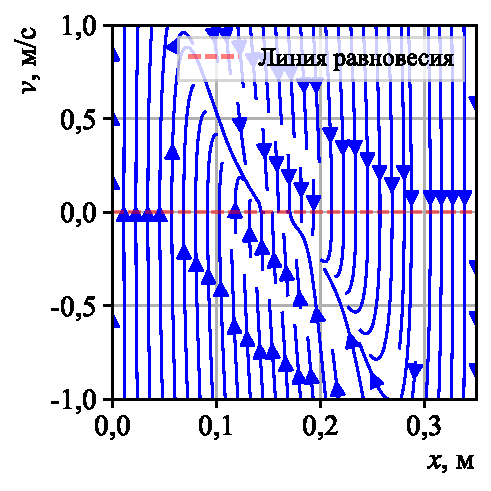
\includegraphics{part3/pp_hold_balanced.pdf} }
		\hfill
		\subcaptionbox{\label{fig:pp_hold_unbalanced}}{
			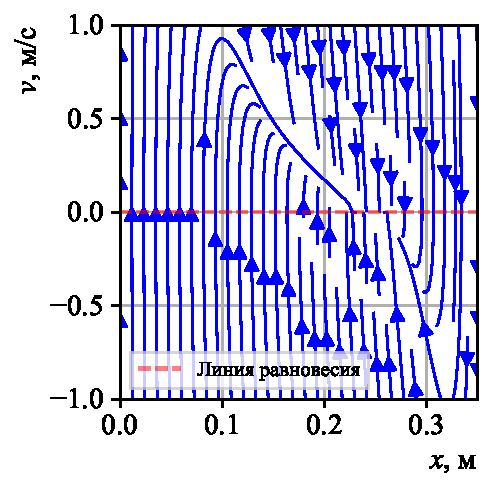
\includegraphics{part3/pp_hold_unbalanced.pdf} }
	}
	\caption{Фазовые портреты при $x_0 = \num{0.15}$ м и различных соотношениях начальных давлений:\\
		а) близкие давления ($p_{1,0} = 3$ бар, $p_{2,0} = 3$ бар);\\
		б) существенная разница ($p_{1,0} = 2$ бар, $p_{2,0} = 4$ бар)}
	\label{fig:pp_hold_matrix}
\end{figure}

Рассмотрение фазовых портретов при различных соотношениях начальных давлений отображенных на  рисунке \ref{fig:pp_hold_matrix} демонстрирует,
что даже при значительной разнице давлений в полостях система сохраняет устойчивое апериодическое движение к положению равновесия.
При близких значениях давлений $p_{1,0}$ и $p_{2,0}$ наблюдается симметричный характер фазовых траекторий. Увеличение разности давлений приводит к незначительной асимметрии траекторий при сохранении общего характера движения.

Математическое описание движения в окрестности положения равновесия может быть получено линеаризацией уравнений движения:

\begin{equation}
	M\ddot{x} + \left(\frac{\gamma p_{1,0}F_1^2}{V_{1,0}} + \frac{\gamma p_{2,0}F_2^2}{V_{2,0}}\right)x + \nu\dot{x} = 0
\end{equation}

где $\nu$ -- коэффициент вязкого трения. Существенное преобладание силы трения над пневматической жёсткостью
($\nu \gg \sqrt{M\left(\frac{\gamma p_{1,0}F_1^2}{V_{1,0}} + \frac{\gamma p_{2,0}F_2^2}{V_{2,0}}\right)}$) обуславливает апериодический характер движения системы.

Проведенный анализ режимов работы электропневматического привода с дискретными распределителями
позволил выявить характерные особенности динамики системы для каждого режима функционирования.
В режиме сильного ускорения [1,0,0,1] наблюдается максимальный перепад давлений между полостями и,
как следствие, наибольшая интенсивность разгона штока с последующим выходом на установившуюся скорость.
Режим умеренного ускорения [1,0,0,0] характеризуется существенным влиянием начальных условий на динамику
системы вследствие политропного изменения состояния воздуха в запертой полости. Режим слабого ускорения
[0,0,0,1] демонстрирует значительную зависимость от сил трения при минимальном перепаде давлений между полостями.
Особую роль играет режим удержания [0,0,0,0], в котором стабилизация положения штока обеспечивается преимущественно
силами трения при апериодическом характере затухания скорости. Построенные фазовые портреты и анализ динамики давлений
позволяют обоснованно подходить к выбору режимов работы при проектировании алгоритмов управления электропневматическим
приводом с дискретными распределителями. При этом учет выявленных закономерностей и особенностей каждого режима позволяет
обеспечить требуемые показатели качества позиционирования при минимизации количества переключений распределителей.
\section{Использование ПИД-регулирования с широтно-импульсной модуляцией}\label{sec:ch3/sec2}

\subsection*{Принципы реализации широтно-импульсной модуляции в пневматических системах с дискретным управлением}\label{subsec:ch3/sec2/sub1}
Широтно-импульсная модуляция (ШИМ) представляет собой метод формирования квазинепрерывного
управляющего воздействия в системах с дискретными исполнительными элементами.
В контексте пневматических систем с дискретными распределителями применение ШИМ
позволяет преодолеть ограничения, связанные с бинарным характером управления, и обеспечить более
точное регулирование положения и скорости исполнительного механизма.

Механизм формирования квазинепрерывного управляющего воздействия
посредством ШИМ основан на периодическом переключении дискретных
распределителей с определенной частотой и скважностью.

Математически это может быть описано следующим образом:

\begin{equation}
	u(t) = \begin{cases}
		1, & 0 \leq t < \alpha T; \\
		0, & \alpha T \leq t < T,
	\end{cases}
\end{equation}
где $u(t)$ -- управляющий сигнал;
$T$ -- период ШИМ;
$\alpha$ -- коэффициент заполнения $0 \leq \alpha \leq 1$.
\nomenclature{$T$}{Период ШИМ}
\nomenclature{$\alpha$}{Коэффициент заполнения\nomrefeqpage}

На рисунке \ref{fig:ch3:pwm_example} показаны временные диаграммы ШИМ-сигнала
с различными значениями коэффициента заполнения.

\begin{figure}[ht]
	\centerfloat{
		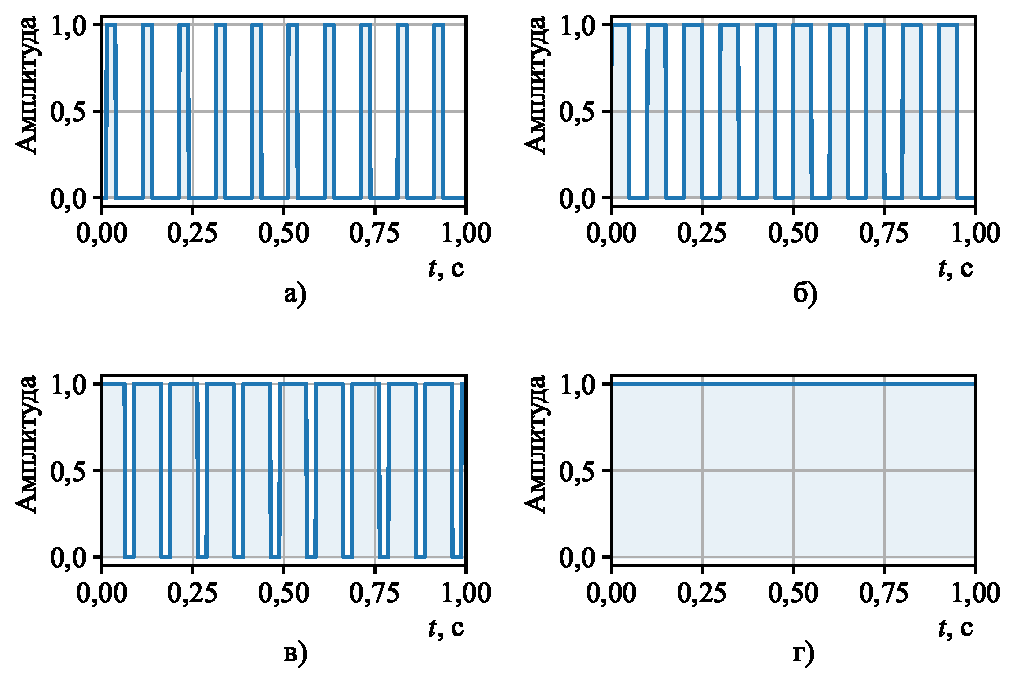
\includegraphics[]{part3/pwm_signal_skewness.pdf}
	}
	\caption{Примеры ШИМ-сигнала с различными значениями коэффициента заполнения:\\
		а) $\alpha = \num{0.3}$; б) $\alpha = \num{0.6}$; в) $\alpha = \num{0.9}$; г) $\alpha = \num{1}$}
	\label{fig:ch3:pwm_example}
\end{figure}

Среднее значение управляющего воздействия за период определяется как:
\begin{equation}
	\bar{u} = \frac{1}{T} \int_0^T u(t) dt = \alpha.
\end{equation}

Влияние частоты ШИМ на динамику пневмопривода является критическим фактором при
проектировании системы управления. С увеличением частоты ШИМ улучшается
гладкость управляющего воздействия, что способствует снижению пульсаций давления
и повышению точности позиционирования. Однако чрезмерно высокая частота может привести
к повышенному износу распределителей и увеличению энергопотребления.

Для анализа влияния частоты ШИМ на динамику системы может быть использована передаточная функция эквивалентного непрерывного звена \cite{pwm_transfer}:
\begin{equation}
	W_{\text{ШИМ}}(s) = \frac{1 - e^{-sT}}{sT},
\end{equation}
где $s$ -- комплексная переменная преобразования Лапласа.
\nomenclature{$W_{\text{ШИМ}}(s)$}{Передаточная функция ШИМ}
\nomenclature{$s$}{Комплексная переменная преобразования Лапласа\nomrefeqpage}
Особенности применения ШИМ для различных типов дискретных
распределителей обусловлены их конструктивными характеристиками и
динамическими свойствами. На рисунке \ref{fig:ch3:pwm_valve_response} показаны рассчитанные
характеристики переходных процессов для распределителя с временем срабатывания $\tau = 30$~мс и различной
частотой ШИМ сигнала.

\begin{figure}[ht]
	\centering
	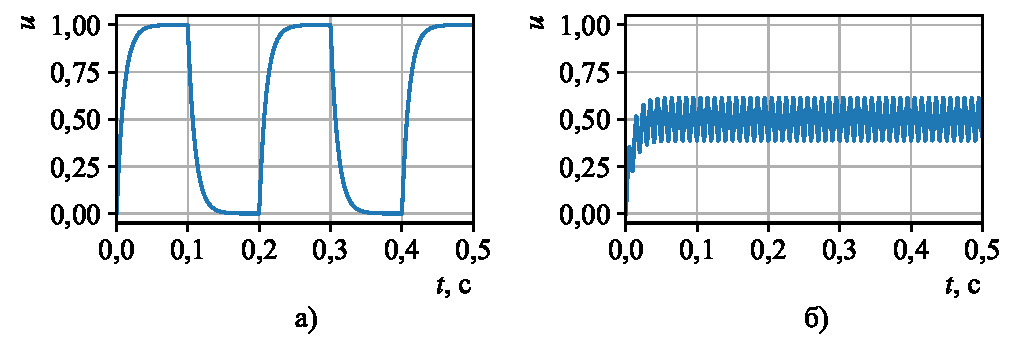
\includegraphics[]{part3/pwm_signal_transfer_function.pdf}
	\caption{Характеристики переходных процессов при различной частоте ШИМ:\\
		а) $f_{\text{ШИМ}} = \num{5}$~Гц; б) $f_{\text{ШИМ}} = \num{100}$~Гц
	}
	\label{fig:ch3:pwm_valve_response}
\end{figure}

При выборе параметров ШИМ необходимо учитывать соотношение между
периодом ШИМ и динамическими характеристиками распределителя:
\begin{equation}
	T_{ШИМ} \geq k\tau_{\text{р}},
\end{equation}
где $\tau_{\text{р}}$ -- время реакции распределителя;
$k$ -- коэффициент запаса (обычно $k \geq 2$).
\nomenclature{$\tau_{\text{р}}$}{Время реакции распределителя\nomrefeqpage}
\nomenclature{$k$}{Коэффициент запаса\nomrefeqpage}

\subsection*{Реализация ПИД-регулирования для пневмоприводов с дискретными распределителями}\label{subsec:ch3/sec2/sub2}

Применение ШИМ в пневмоприводах с дискретными распределителями открывает
возможность использования алгоритмов управления,
изначально разработанных для непрерывных систем.
Одним из наиболее эффективных и широко применяемых методов является
пропорционально-интегрально-дифференциальное (ПИД) регулирование.

Структура ПИД-регулятора для пневмопривода
с дискретными распределителями представлена на рисунке \ref{fig:ch3:pid_pwm_control}.

\begin{figure}[ht]
	\centering
	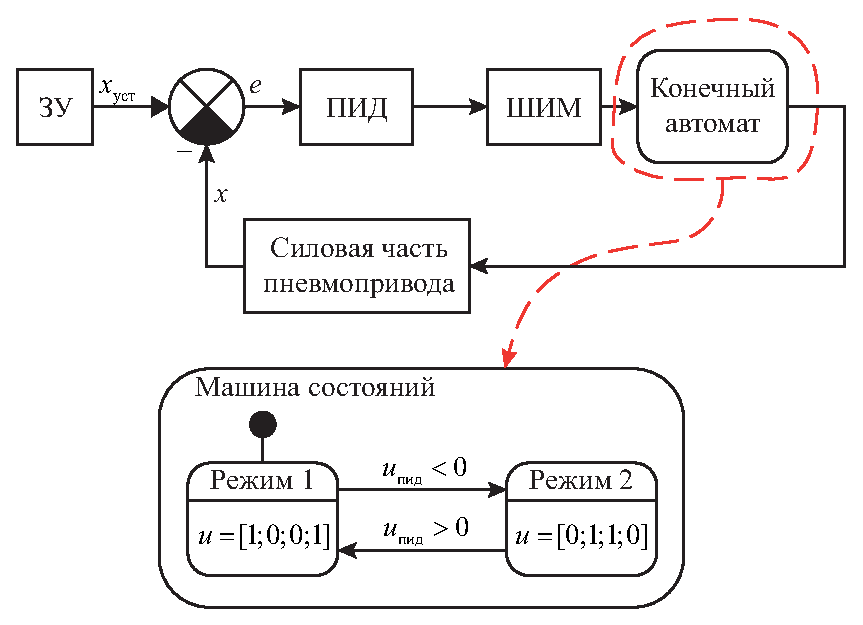
\includegraphics[]{part3/pid_pwm.eps}
	\caption{Структурная схема ПИД-регулятора с ШИМ управлением}
	\label{fig:ch3:pid_pwm_control}
\end{figure}

В данной схеме выходной сигнал ПИД-регулятора преобразуется в коэффициент
заполнения ШИМ, который управляет дискретными распределителями
пневмопривода. Этот подход позволяет достичь высокой точности
управления, характерной для непрерывных систем, в условиях
дискретного исполнительного механизма.

Математическая модель ПИД-регулятора в непрерывной форме описывается уравнением \cite{pid_pwm}:
\begin{equation}\label{eq:pid_base}
	u_{\text{пид}}(t) = K_{\text{п}} e(t) + K_{\text{и}} \int_0^t e(\tau)d\tau + K_{\text{д}}\frac{de(t)}{dt},
\end{equation}
где
$e(t)$ -- ошибка регулирования;
$K_\text{п}$, $K_\text{и}$, $K_\text{д}$ -- коэффициенты пропорциональной, интегральной и
дифференциальной составляющих соответственно;
\nomenclature{$K_\text{п}$}{Коэффициент пропорциональной составляющей\nomrefeqpage}
\nomenclature{$K_\text{и}$}{Коэффициент интегральной составляющей\nomrefeqpage}
\nomenclature{$K_\text{д}$}{Коэффициент дифференциальной составляющей\nomrefeqpage}
\nomenclature{$e(t)$}{Ошибка регулирования}

Выходной сигнал ПИД-регулятора преобразуется в коэффициент заполнения ШИМ согласно формуле:
\begin{equation}
	\alpha = \frac{u(i) + u_{max}}{2u_{max}},
\end{equation}
где $u_{max}$ -- максимальное значение управляющего сигнала.
\nomenclature{$\alpha$}{Коэффициент заполнения ШИМ\nomrefeqpage}
\nomenclature{$u_{max}$}{Максимальное значение управляющего сигнала\nomrefeqpage}

Однако в рассматриваемой конфигурации пневмопривода с дискретными распределителями
выходной сигнал ПИД-регулятора, как сказано выше, преобразуется в бинарное
управляющее воздействие посредством ШИМ. При этом возможна реализация
только двух основных режимов движения: выдвижение штока и его втягивание.

Математически это может быть описано следующим образом:

\begin{equation}
	\mathbf{u}(t) = \begin{cases}
		[1,0,0,1], & \text{если } u_\text{пид}(t) > 0; \\
		[0,1,1,0], & \text{если } u_\text{пид}(t) < 0,
	\end{cases}
\end{equation}
где $u_\text{пид}(t)$ -- выходной сигнал ПИД-регулятора.
\nomenclature{$u_\text{пид}(t)$}{Выходной сигнал ПИД-регулятора\nomrefeqpage}

Для данного случая, выходной сигнал ПИД-регулятора
преобразуется в коэффициент заполнения ШИМ согласно формуле:

\begin{equation}
	\alpha = \begin{cases}
		\frac{u_\text{ПИД}(t)}{u_{max}},  & \text{если } u_\text{ПИД}(t) > 0; \\
		-\frac{u_\text{ПИД}(t)}{u_{max}}, & \text{если } u_\text{ПИД}(t) < 0,
	\end{cases}
\end{equation}
где $u_{max}$ -- максимальное значение управляющего сигнала.

Проанализированные в дальнейших главах переходные процессы при изменении различных
параметров, и эти исследования показали, что в широком диапазоне
изменения параметров переходный процесс носит колебательный характер. В основном это связано с
тем, что при использовании ШИМ рассматривается только два состояния: выдвижение и втягивание.
В результате этого возникает резкое изменение давления в камерах распределителя, что приводит к возникновению
колебаний в системе. Данное ограничение является одной из ключевых причин для рассмотрения модифицированных
структур управления, способных обеспечить более эффективное торможение и позиционирование
привода за счет использования дополнительных режимов работы распределителей или реализации
торможения.

\subsection*{Модифицированная структура ПИД-регулятора}\label{subsec:ch3/sec2/sub3}

Как было показано выше, классическая структура ПИД-регулятора с ШИМ управлением имеет
существенные ограничения в обеспечении эффективного управления пневмоприводом с
дискретными распределителями. Основным недостатком является отсутствие прямого управления режимом торможения,
что приводит к значительному перерегулированию и колебательности системы. Для преодоления данных ограничений
предлагается модифицированная структура ПИД-регулятора, обеспечивающая адаптивное торможение на основе анализа динамического состояния системы.

Предложенная модификация базируется на концепции прогнозирования тормозного пути и формировании упреждающего
управляющего воздействия. Математическая модель модифицированного ПИД-регулятора включает три основных компонента:
классический ПИД-регулятор, описанный выражением \eqref{eq:pid_base}, блок прогнозирования тормозного пути и блок формирования тормозного воздействия.

Прогнозирование тормозного пути осуществляется на основе анализа кинетической энергии системы и желаемого ускорения торможения:

\begin{equation}\label{eq:braking_prediction}
	s_{\text{торм}}(t) = \frac{v(t)|v(t)|}{2a_{\text{торм}}} + \frac{K_{\text{б}}v(t)^2}{2},
\end{equation}
где $v(t)$ -- текущая скорость привода;
$a_{\text{торм}}$ -- желаемое ускорение торможения;
$K_{\text{б}}$ -- коэффициент запаса по тормозному пути, учитывающий инерционность пневматической системы.
\nomenclature{$s_{\text{торм}}(t)$}{Прогнозируемое тормозное расстояние\nomrefeqpage}
\nomenclature{$a_{\text{торм}}$}{Желаемое ускорение торможения\nomrefeqpage}
\nomenclature{$K_{\text{б}}$}{Коэффициент запаса по тормозному пути\nomrefeqpage}


Для учета нелинейных свойств пневматической системы в расчете тормозного пути вводится дополнительный экспоненциальный множитель:

\begin{equation}\label{eq:modified_braking_distance}
	s_{\text{торм}}(t) = \frac{v(t)|v(t)|}{2a_{\text{торм}}} \cdot \left(1 + K_\text{нл} \cdot e^{-\frac{|v(t)|}{v_\text{хар}}}\right),
\end{equation}
где $K_\text{нл}$ -- коэффициент нелинейности;
$v_\text{хар}$ -- характерная скорость, определяющая влияние нелинейности.
\nomenclature{$K_\text{нл}$}{Коэффициент нелинейности\nomrefeqpage}
\nomenclature{$v_\text{хар}$}{Характерная скорость\nomrefeqpage}

Эффективность торможения определяется соотношением между прогнозируемым
тормозным путем и расстоянием до целевой точки. Коэффициент интенсивности торможения вычисляется с использованием нелинейной функции:

\begin{equation}\label{eq:braking_intensity_expanded}
	k_{\text{торм}}(t) = \begin{cases}
		\left(1 - \min\left(\frac{s_{\text{цель}}(t)}{s_{\text{торм}}(t) \cdot k_{\text{порог}}}, 1\right)\right)^2 \cdot \eta(v), & |v(t)| > v_{\text{порог}};   \\
		0,                                                                                                                         & |v(t)| \leq v_{\text{порог}},
	\end{cases}
\end{equation}
где $s_{\text{цель}}(t) = |x_{\text{зад}} - x(t)|$ -- расстояние до целевой точки;
$k_{\text{порог}}$ -- пороговый коэффициент начала торможения;
$\eta(v)$ -- функция модуляции интенсивности торможения:

\begin{equation}\label{eq:modulation_function}
	\eta(v) = 1 - \exp\left(-\left(\frac{|v(t)|}{v_{\text{хар}}}\right)^2\right),
\end{equation}
где $v_{\text{хар}}$ -- характерная скорость, определяющая форму функции модуляции.
\nomenclature{$\eta(v)$}{Функция модуляции интенсивности торможения\nomrefeqpage}

В практической реализации для обеспечения более плавного перехода к режиму торможения и выхода из него применяется сигмоидальная функция:

\begin{equation}\label{eq:sigmoid_braking}
	k_{\text{торм}}(t) = \frac{1}{1 + e^{5\left(\frac{s_{\text{цель}}(t)}{s_{\text{торм}}(t) \cdot k_{\text{порог}}} - 0.5\right)}}.
\end{equation}

Данная функция обеспечивает плавное нарастание интенсивности торможения при приближении к целевой позиции и снижение при удалении от нее.

Для обеспечения устойчивости переключения между режимами движения и торможения вводится гистерезисная характеристика активации торможения:

\begin{equation}\label{eq:hysteresis}
	v_{\text{порог}}(t) = v_{\text{порог}}^0 \cdot \begin{cases}
		1 + \Delta v, & \text{при переходе к торможению}; \\
		1 - \Delta v, & \text{при выходе из торможения},
	\end{cases}
\end{equation}
где $v_{\text{порог}}^0$ -- базовое пороговое значение скорости;
$\Delta v$ -- ширина гистерезиса.
\nomenclature{$v_{\text{порог}}(t)$}{Пороговое значение скорости\nomrefeqpage}
\nomenclature{$\Delta v$}{Ширина гистерезиса\nomrefeqpage}

Результирующее управляющее воздействие формируется путем
взвешенной комбинации сигналов ПИД-регулятора и тормозного контура:

\begin{equation}\label{eq:combined_control}
	u_{\text{м}}(t) = (1 - k_{\text{торм}}(t))u_{\text{пид}}(t) + k_{\text{торм}}(t)u_{\text{торм}}(t),
\end{equation}
где $u_{\text{торм}}(t)$ -- сигнал управления в режиме торможения, определяемый направлением движения:
\nomenclature{$u_{\text{торм}}(t)$}{Сигнал управления в режиме торможения\nomrefeqpage}

\begin{equation}\label{eq:braking_control_expanded}
	\mathbf{u}_{\text{торм}}(t) = \begin{cases}
		[0, \alpha{\text{т}}(t), \alpha_{\text{т}}(t), 0],  & v(t) > v_{\text{порог}};      \\
		[\alpha_{\text{т}}(t), 0, 0, \alpha_{\text{т}}(t)], & v(t) < -v_{\text{порог}};     \\
		[0, 0, 0, 0],                                       & |v(t)| \leq v_{\text{порог}}.
	\end{cases}
\end{equation}

Коэффициент заполнения ШИМ в режиме торможения вычисляется с учетом динамических характеристик системы:

\begin{equation}\label{eq:braking_pwm_expanded}
	\alpha_{\text{т}}(t) = k_{\text{торм}}(t) \cdot \alpha_{\text{макс}} \cdot \left(1 + K_{\text{к}}\frac{d|v(t)|}{dt}\right),
\end{equation}
где $K_{\text{к}}$ -- коэффициент коррекции, учитывающий скорость изменения модуля скорости.
\nomenclature{$K_{\text{к}}$}{Коэффициент коррекции\nomrefeqpage}

Для повышения устойчивости системы к колебаниям при малых скоростях вблизи целевой позиции
реализовано активное демпфирование. Логика активного демпфирования заключается в формировании
управляющего воздействия, противодействующего текущему направлению движения:

\begin{equation}\label{eq:active_damping}
	\mathbf{u}_{\text{демп}}(t) = \begin{cases}
		[0, \alpha_{\text{д}}(t), 0, 0], & v(t) > 0;                     \\
		[0, 0, \alpha_{\text{д}}(t), 0], & v(t) < 0;                     \\
		[\alpha_{\text{д}}(t), 0, 0, 0], & v(t) = 0 \text{ и } e(t) > 0; \\
		[0, 0, 0, \alpha_{\text{д}}(t)], & v(t) = 0 \text{ и } e(t) < 0,
	\end{cases}
\end{equation}
где $\alpha_{\text{д}}(t) = K_{\text{д}} \cdot |v(t)| \cdot \alpha_{\text{макс}}$ -- коэффициент заполнения ШИМ для демпфирования;
$K_{\text{д}}$ -- коэффициент демпфирования;
$e(t)$ -- ошибка позиционирования.

Дополнительно в модифицированной структуре ПИД-регулятора реализован механизм защиты от
интегрального насыщения, который адаптивно ограничивает скорость нарастания
интегральной составляющей при насыщении управляющего сигнала:

\begin{equation}\label{eq:anti_windup}
	I(t) = \begin{cases}
		I(t-1) + K_{\text{и}} \cdot e(t) \cdot \Delta t \cdot \gamma, & \text{при насыщении};  \\
		I(t-1) + K_{\text{и}} \cdot e(t) \cdot \Delta t,              & \text{в иных случаях},
	\end{cases}
\end{equation}
где $I(t)$ -- интегральная составляющая;
$\gamma$ -- коэффициент снижения скорости интегрирования ($\gamma < 1$);
$\Delta t$ -- интервал дискретизации.
\nomenclature{$\gamma$}{Коэффициент снижения скорости интегрирования\nomrefeqpage}
\nomenclature{$\Delta t$}{Интервал дискретизации\nomrefeqpage}

Для фильтрации высокочастотных шумов в дифференциальной составляющей применяется экспоненциальный фильтр:

\begin{equation}\label{eq:derivative_filter}
	D(t) = \alpha \cdot \frac{e(t) - e(t-1)}{\Delta t} + (1-\alpha) \cdot D(t-1),
\end{equation}
где $D(t)$ -- отфильтрованная дифференциальная составляющая;
$\alpha$ -- коэффициент фильтрации ($0 < \alpha < 1$).
\nomenclature{$\alpha$}{Коэффициент фильтрации\nomrefeqpage}

Данный алгоритм был зарегистрирован в качестве программы для ЭВМ \cite{progbib1}.

Исследование динамических характеристик системы управления электропневматическим приводом демонстрирует существенные различия в характере
переходных процессов для классической и модифицированной структур ПИД-регулятора с ШИМ.

Для классической структуры характерно наличие значительной колебательности, обусловленной отсутствием эффективного
управления торможением. Это проявляется в перерегулировании при подходе к заданной позиции и возникновении затухающих или авто-колебаний
из-за ограниченности режимов работы распределителей.

Модифицированная структура обеспечивает более качественный переходный процесс благодаря адаптивному торможению и
прогнозированию тормозного пути.

\begin{figure}
	\centering
	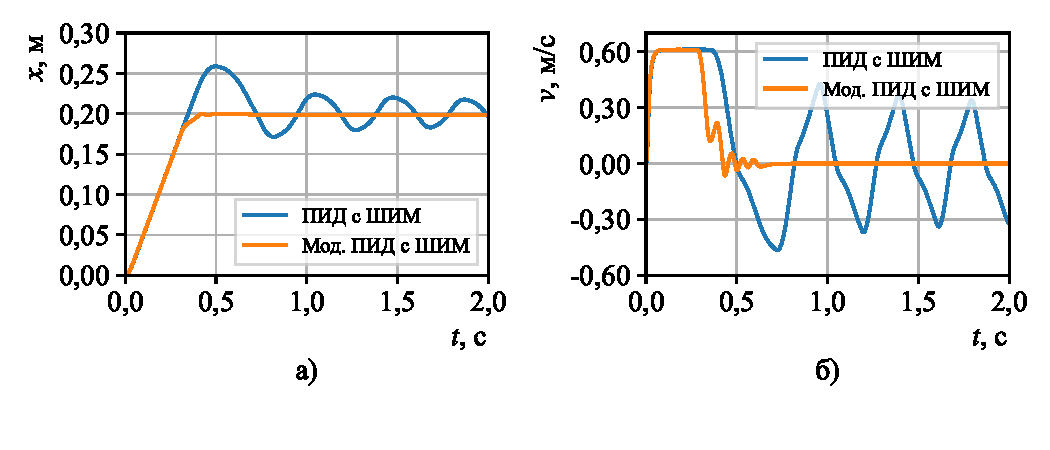
\includegraphics[]{part3/pid_comparison_2.pdf}
	\caption{Сравнение переходных процессов для классической и модифицированной структур ПИД-регулятора с ШИМ управлением:\\
		а) позиционирование штока; б) скорость штока}
	\label{fig:ch3:transient_comparison}
\end{figure}

Представленные на рисунке \ref{fig:ch3:transient_comparison} результаты наглядно демонстрируют преимущества
модифицированной структуры в обеспечении качества позиционирования пневмопривода. Предложенная структура
позволяет существенно снизить колебательность процесса и устранить перерегулирование при сохранении приемлемой статической точности позиционирования.
Внедрение механизмов прогнозирования тормозного пути, активного демпфирования и защиты от интегрального насыщения обеспечивает
робастность системы к параметрическим возмущениям и изменениям динамических характеристик пневмопривода.

\section{Использование управления в скользящих режимах}\label{sec:ch3/sec3}

\subsection*{Теоретические основы управления в скользящих режимах}\label{subsec:ch3/sec3/sub1}

Управление в скользящих режимах представляет собой метод управления нелинейными системами, который особенно
эффективен в условиях неопределенностей и нелинейностей, характерных для пневматических систем.
Концепция данного метода основана на принудительном переводе рабочей точки динамической
системы на заранее заданную поверхность в пространстве состояний
и последующем удержании её в окрестности этой поверхности.

Представим физический смысл данного подхода на примере позиционного пневмопривода.
Допустим, мы хотим переместить шток пневмоцилиндра из текущего положения $x$ в заданное $x_d$.
Состояние системы в любой момент времени можно охарактеризовать двумя параметрами:
ошибкой позиционирования $e = x_d - x$ и скоростью изменения этой ошибки $\dot{e} = -\dot{x}$
(т.е. скоростью движения штока с обратным знаком). На фазовой плоскости $(e, \dot{e})$ текущее состояние системы изображается
точкой, а её движение – траекторией, согласно рисунку~\ref{fig:phase_plane}.

\begin{figure}[ht]
	\centerfloat{
		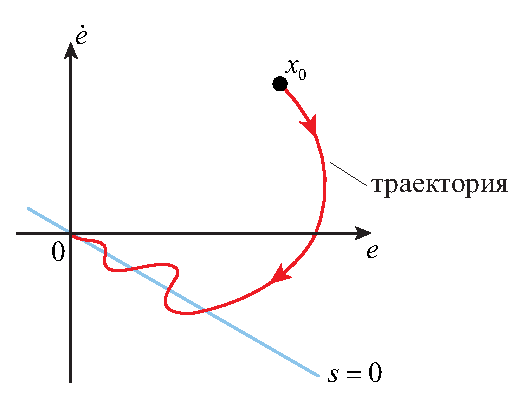
\includegraphics[]{part3/phase_plane.eps}
	}
	\caption{Иллюстрация принципа управления в скользящих режимах: $s=0$ -- поверхность скольжения; $S^+$ и $S^-$ -- области притяжения к поверхности скольжения}
	\label{fig:phase_plane}
\end{figure}

Ключевая идея управления в скользящих режимах заключается в
определении на фазовой плоскости линии (или в общем случае многомерной поверхности), называемой \textit{поверхностью скольжения}, которая описывается уравнением:
\begin{equation}
	s(e, \dot{e}) = 0,
\end{equation}
где $s(e, \dot{e})$ -- некоторая функция, связывающая ошибку позиционирования и скорость.
\nomenclature{$s(e, \dot{e})$}{Функция поверхности скольжения\nomrefeqpage}

Наиболее простой случай -- линейная функция:
\begin{equation}
	s = \dot{e} + \lambda e,
\end{equation}
где $\lambda > 0$ -- параметр, определяющий скорость сходимости ошибки к нулю.
\nomenclature{$\lambda$}{Параметр скорости сходимости ошибки к нулю\nomrefeqpage}

После определения функции $s$ вся фазовая плоскость делится на
две области: $s > 0$ и $s < 0$. Для каждой из этих областей выбирается своё управляющее
воздействие, которое принудительно направляет траекторию системы к поверхности скольжения. Когда траектория достигает
поверхности, система начинает двигаться вдоль неё к состоянию с нулевой ошибкой $(e, \dot{e}) = (0, 0)$.

В случае пневмопривода с дискретными распределителями можно использовать следующий закон управления:
\begin{equation}
	\mathbf{u} = \begin{cases}
		[1,0,0,1], & s > \varepsilon;      \\
		[0,0,0,0], & |s| \leq \varepsilon; \\
		[0,1,1,0], & s < -\varepsilon,
	\end{cases}
\end{equation}
где $\varepsilon > 0$ -- малый параметр, определяющий ширину «коридора» вокруг поверхности скольжения; $[1,0,0,1]$ -- комбинация состояний
распределителей, обеспечивающая максимальное ускорение в положительном направлении; $[0,1,1,0]$ -- комбинация, обеспечивающая максимальное
ускорение в отрицательном направлении; $[0,0,0,0]$ -- все распределители закрыты.
\nomenclature{$\varepsilon$}{Малый параметр, определяющий ширину <<коридора>> вокруг поверхности скольжения\nomrefeqpage}

При движении к поверхности скольжения выбирается режим максимального ускорения (положительного или отрицательного, в зависимости
от знака $s$). Когда система попадает в $\varepsilon$-окрестность поверхности ($|s| \leq \varepsilon$), все распределители закрываются,
что приводит к торможению штока под действием сил трения и пневматической жёсткости (сжатый воздух в закрытых полостях действует как пружина).

Этот принцип управления обеспечивает робастность (устойчивость к возмущениям) и простоту реализации, что делает его особенно
привлекательным для систем с дискретными исполнительными элементами, такими как пневмоприводы с дискретными распределителями.

\subsection*{Многорежимное управление в скользящих режимах}\label{subsec:ch3/sec3/sub2}

При практической реализации управления в скользящих режимах для пневмопривода с дискретными распределителями возникает
ряд проблем, связанных с динамикой системы. Базовая трёхрежимная схема, хотя и обеспечивает достижение целевого положения,
но может приводить к возникновению колебаний вблизи заданной позиции, что снижает точность позиционирования и увеличивает износ распределителей.

Для преодоления этих недостатков предлагается использовать многорежимное управление (5 и 7 режимов), обеспечивающее
более плавное торможение при подходе к целевому положению. В данном разделе рассматриваются особенности
таких схем управления и их преимущества по сравнению с базовой трёхрежимной схемой.

\textbf{Трёхрежимное управление.}
Базовая схема управления в скользящих режимах для пневмопривода с дискретными распределителями предусматривает три режима работы:
\begin{enumerate}
	\item \textbf{Режим максимального положительного ускорения} $[1,0,0,1]$: поршневая полость соединена с источником питания, штоковая -- с атмосферой. Этот режим обеспечивает максимальное ускорение штока в положительном направлении.
	\item \textbf{Режим максимального отрицательного ускорения} $[0,1,1,0]$: поршневая полость соединена с атмосферой, штоковая -- с источником питания. Этот режим обеспечивает максимальное ускорение штока в отрицательном направлении.
	\item \textbf{Режим удержания} $[0,0,0,0]$: обе полости изолированы от источника питания и атмосферы. Этот режим обеспечивает торможение и удержание штока за счёт пневматической жёсткости и сил трения.
\end{enumerate}

Закон переключения между режимами определяется значением функции переключения $s = \dot{e} + \lambda e$:
\begin{equation}
	\mathbf{u}(s) = \begin{cases}
		[1,0,0,1], & s > \varepsilon;      \\
		[0,0,0,0], & |s| \leq \varepsilon; \\
		[0,1,1,0], & s < -\varepsilon,
	\end{cases}
\end{equation}
где $\varepsilon > 0$ -- параметр, определяющий ширину зоны переключения.
\nomenclature{$\varepsilon$}{Ширина зоны переключения\nomrefeqpage}

В фазовом пространстве векторное поле системы разделяется на три области линией переключения $s = 0$, представленные на рисунке~\ref{fig:vector_field_linear}.
В области $s > \varepsilon$ векторы скоростей направлены к линии переключения под действием управления $\mathbf{u} = [1,0,0,1]$.
При $s < -\varepsilon$ управление $\mathbf{u} = [0,1,1,0]$ формирует векторное поле, обеспечивающее движение к линии
переключения с противоположной стороны. В зоне $|s| \leq \varepsilon$ все распределители закрыты $\mathbf{u} = [0,0,0,0]$, что приводит к замедлению движения.

\begin{figure}[ht]
	\centering
	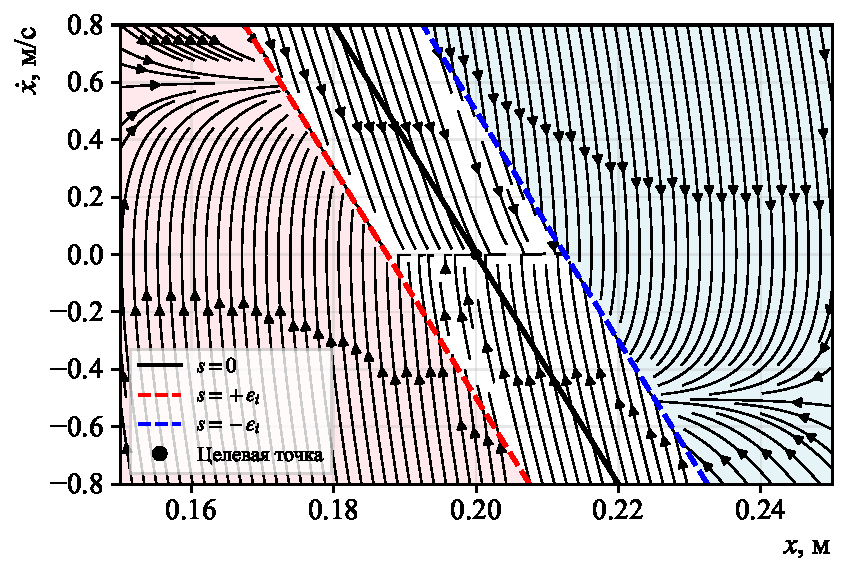
\includegraphics[]{part3/phase_portrait_3mode.pdf}
	\caption{Распределение векторного поля в фазовом пространстве для трёхрежимного управления. Стрелками показаны направления
		движения в различных областях фазовой плоскости, пунктирными линиями -- границы переключения режимов}
	\label{fig:vector_field_linear}
\end{figure}

При малых значениях параметра $\varepsilon$ в системе может возникать эффект <<дребезга>> (chattering),
обусловленный конечным быстродействием электромагнитных распределителей и инерционностью процессов.
На рисунке~\ref{fig:ch3:transient_comparison_linear_mode3} представлены результаты моделирования
для двух значений параметра $\varepsilon$.

\begin{figure}[ht]
	\centering
	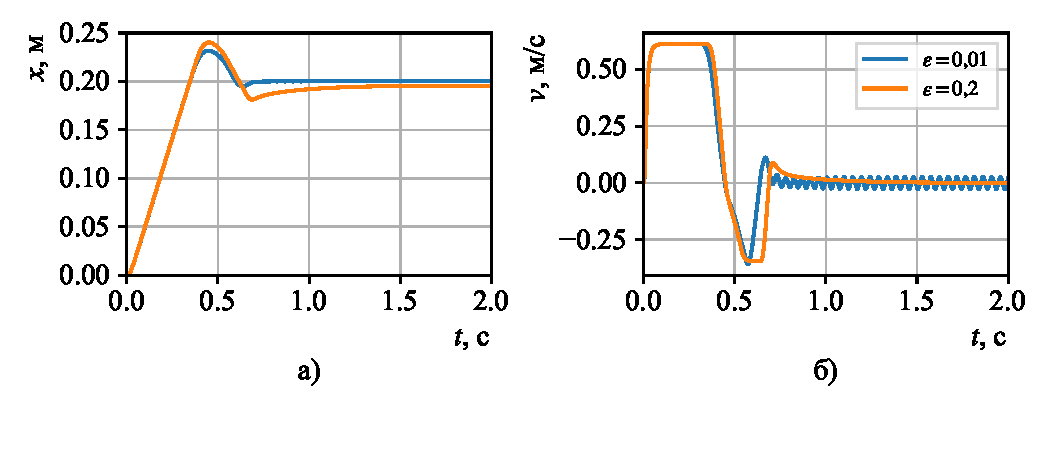
\includegraphics[]{part3/sliding_mode_linear_transients.pdf}
	\caption{Переходные процессы для трёхрежимного управления с различными значениями параметра $\varepsilon$.
		При малом значении $\varepsilon = \num{0.01}$ (синяя линия) наблюдаются колебания,
		при большем значении $\varepsilon = \num{0.2}$ (красная линия) процесс становится апериодическим, но с большей статической ошибкой}
	\label{fig:ch3:transient_comparison_linear_mode3}
\end{figure}

Ключевое ограничение трёхрежимного управления заключается в компромиссе между точностью
позиционирования и стабильностью процесса. Увеличение параметра $\varepsilon$ позволяет устранить колебания,
но приводит к росту статической ошибки, ограниченной соотношением $|e_{ss}| \leq \varepsilon/\lambda$. Уменьшение $\varepsilon$
повышает теоретическую точность, но вызывает колебания, что на практике может даже снизить фактическую точность позиционирования.

\textbf{Пятирежимное управление.}
Для преодоления ограничений трёхрежимной схемы предлагается пятирежимное управление,
которое вводит дополнительные промежуточные режимы торможения. Закон управления имеет вид:
\begin{equation}\label{eq:control_law_5_mode}
	\mathbf{u}(s) = \begin{cases}
		[1,0,0,1], & s > \varepsilon_2;                      \\
		[1,0,0,0], & \varepsilon_1 < s \leq \varepsilon_2;   \\
		[0,0,0,0], & |s| \leq \varepsilon_1 ;                \\
		[0,0,1,0], & -\varepsilon_2 < s \leq -\varepsilon_1; \\
		[0,1,1,0], & s \leq -\varepsilon_2,
	\end{cases}
\end{equation}
где $\varepsilon_1, \varepsilon_2$ -- параметры, определяющие границы зон переключения режимов ($\varepsilon_1 < \varepsilon_2$).

Дополнительные режимы $[1,0,0,0]$ и $[0,0,1,0]$ обеспечивают умеренное ускорение в положительном и отрицательном направлениях соответственно.
Их действие заключается в создании более плавного торможения перед переходом в режим удержания.
Векторное поле в фазовом пространстве для пятирежимного управления показано на рис.~\ref{fig:vector_field_linear_5mode}.

\begin{figure}[ht]
	\centering
	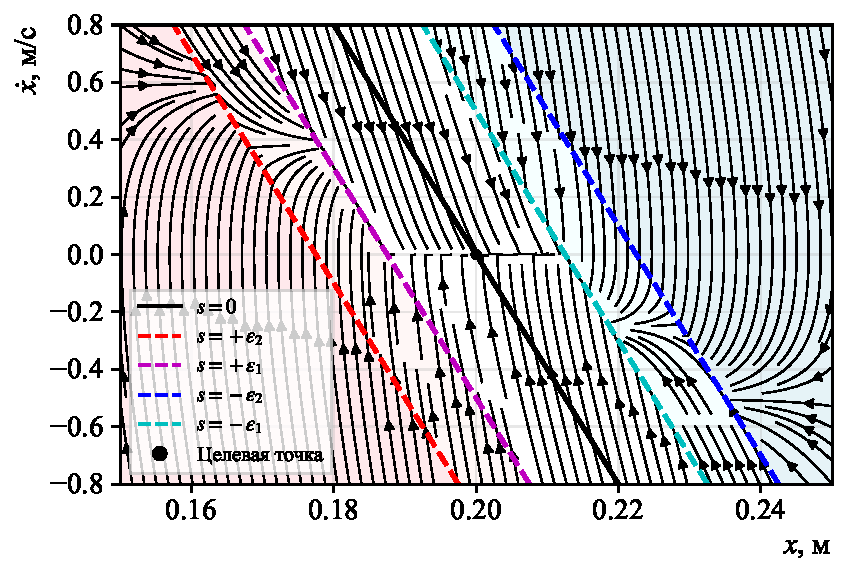
\includegraphics[]{part3/phase_portrait_5mode.pdf}
	\caption{Распределение векторного поля в фазовом пространстве для пятирежимного управления.
		Введение дополнительных режимов торможения создаёт более сложную структуру векторного поля с промежуточными зонами управления}
	\label{fig:vector_field_linear_5mode}
\end{figure}

Ключевое преимущество пятирежимного управления заключается в более плавном снижении скорости движения перед
включением режима удержания. Это позволяет уменьшить перерегулирование и снизить статическую ошибку без увеличения
частоты переключений. Также снижается вероятность возникновения «дребезга», поскольку система проходит
через промежуточные режимы торможения, что сглаживает переходы между режимами.

\textbf{Семирежимное управление.}
Дальнейшее развитие концепции многорежимного управления привело к разработке семирежимной схемы,
обеспечивающей ещё более тонкую градацию торможения перед достижением целевого положения.
Закон управления имеет вид:
\begin{equation}\label{eq:control_law_7_mode}
	\mathbf{u}(s) = \begin{cases}
		[1,0,0,1], & s > \varepsilon_3                     ; \\
		[1,0,0,0], & \varepsilon_2 < s \leq \varepsilon_3 ;  \\
		[0,0,0,1], & \varepsilon_1 < s \leq \varepsilon_2 ;  \\
		[0,0,0,0], & |s| \leq \varepsilon_1          ;       \\
		[0,1,0,0], & -\varepsilon_2 < s \leq -\varepsilon_1; \\
		[0,0,1,0], & -\varepsilon_3 < s \leq -\varepsilon_2; \\
		[0,1,1,0], & s \leq -\varepsilon_3,
	\end{cases}
\end{equation}
где $\varepsilon_1, \varepsilon_2, \varepsilon_3$ -- параметры, определяющие границы зон переключения режимов ($\varepsilon_1 < \varepsilon_2 < \varepsilon_3$).

Дополнительные режимы $[0,0,0,1]$ и $[0,1,0,0]$ обеспечивают слабое ускорение в положительном и
отрицательном направлениях, создавая ещё более плавный переход к режиму удержания. Векторное поле
в фазовом пространстве для семирежимного управления показано на рис.~\ref{fig:vector_field_linear_7mode}.

\begin{figure}[ht]
	\centering
	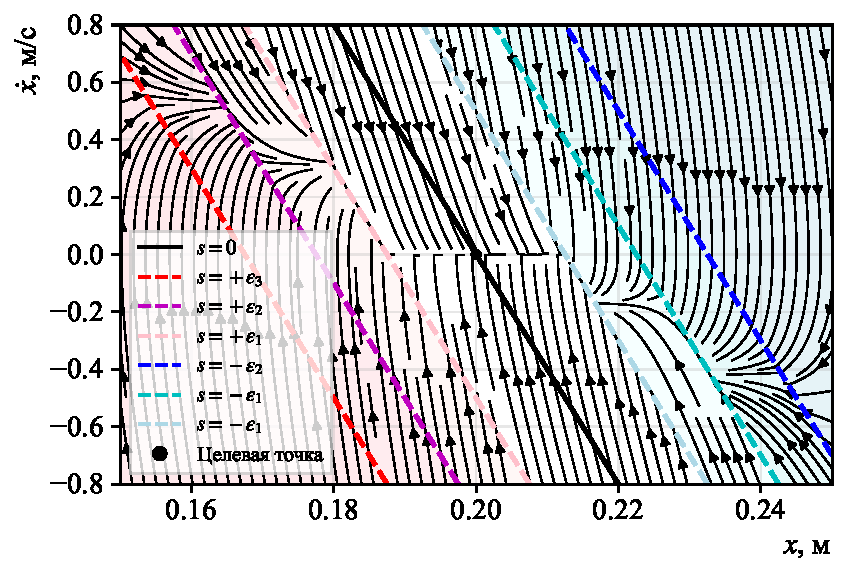
\includegraphics[]{part3/phase_portrait_7mode.pdf}
	\caption{Распределение векторного поля в фазовом пространстве для семирежимного управления.
		Градация режимов торможения создаёт более сложную, но эффективную структуру векторного поля
		с несколькими промежуточными зонами}
	\label{fig:vector_field_linear_7mode}
\end{figure}

Семирежимное управление обеспечивает наиболее плавное снижение скорости перед остановкой, что позволяет
достичь высокой точности позиционирования при минимальном количестве переключений распределителей.
Как показали результаты моделирования (подробнее в главе~\ref{ch:ch5}), данная схема обеспечивает наилучшее
сочетание точности позиционирования, быстродействия и ресурсных показателей по сравнению с трёх- и пятирежимным управлением.

\subsection*{Типы поверхностей скольжения}\label{subsec:ch3/sec3/sub3}

Эффективность управления в скользящих режимах существенно зависит от выбора поверхности скольжения.
В данном исследовании рассматриваются два основных типа поверхностей: интегральная и терминальная.

\textbf{Интегральная поверхность скольжения.}
Интегральная поверхность скольжения описывается уравнением \cite{sliding_surface_integral}:
\begin{equation}
	s_I = \dot{e} + \lambda_1 e + \lambda_2 \int_0^t e(\tau)d\tau,
\end{equation}
где $\lambda_1$ и $\lambda_2$ -- положительные коэффициенты.

Главное отличие интегральной поверхности от линейной заключается в наличии интегральной составляющей,
которая обеспечивает нулевую статическую ошибку в установившемся режиме. Это особенно важно для
позиционных систем, где требуется высокая точность позиционирования.

При движении вдоль интегральной поверхности динамика ошибки описывается дифференциальным уравнением второго порядка:
\begin{equation}
	\ddot{e} + \lambda_1 \dot{e} + \lambda_2 e = 0.
\end{equation}

Характер переходного процесса зависит от соотношения коэффициентов $\lambda_1$ и $\lambda_2$:
\begin{itemize}
	\item при $\lambda_1^2 > 4\lambda_2$ система демонстрирует апериодический характер движения;
	\item при $\lambda_1^2 < 4\lambda_2$ -- колебательный процесс;
	\item при $\lambda_1^2 = 4\lambda_2$ -- критический апериодический процесс (оптимальное соотношение).
\end{itemize}

\textbf{Терминальная поверхность скольжения.}
Терминальная поверхность скольжения представляется выражением \cite{sliding_surface_terminal}:
\begin{equation}
	s_T = \dot{e} + \beta |e|^{q/p} \text{sign}(e),
\end{equation}
где $p$ и $q$ -- нечетные числа, удовлетворяющие условию $1 < q/p < 2$; $\beta$ -- положительный коэффициент.

Главная особенность терминальной поверхности -- обеспечение конечного времени сходимости ошибки к нулю.
При движении вдоль терминальной поверхности динамика ошибки описывается нелинейным дифференциальным уравнением:
\begin{equation}
	\dot{e} = -\beta |e|^{q/p} \text{sign}(e).
\end{equation}

Время сходимости ошибки к нулю можно вычислить аналитически:
\begin{equation}
	T_f = \frac{p}{\beta(p-q)}|e(0)|^{1-q/p}.
\end{equation}

Ключевое преимущество терминальной поверхности -- ускорение сходимости при малых ошибках.
Поскольку $q/p > 1$, то при $e \to 0$ скорость сходимости ошибки увеличивается, что обеспечивает
более быстрое достижение целевого положения по сравнению с линейной или интегральной поверхностями.
Это особенно важно для прецизионных систем, где требуется высокая точность позиционирования.

На рис.~\ref{fig:smc_terminal} представлены результаты моделирования системы с терминальной
поверхностью скольжения при $p = 9$, $q = 11$ и $\beta = 5$. Как видно из графиков, система
быстро достигает целевого положения без перерегулирования, демонстрируя высокую точность позиционирования.

\begin{figure}[ht]
	\centering
	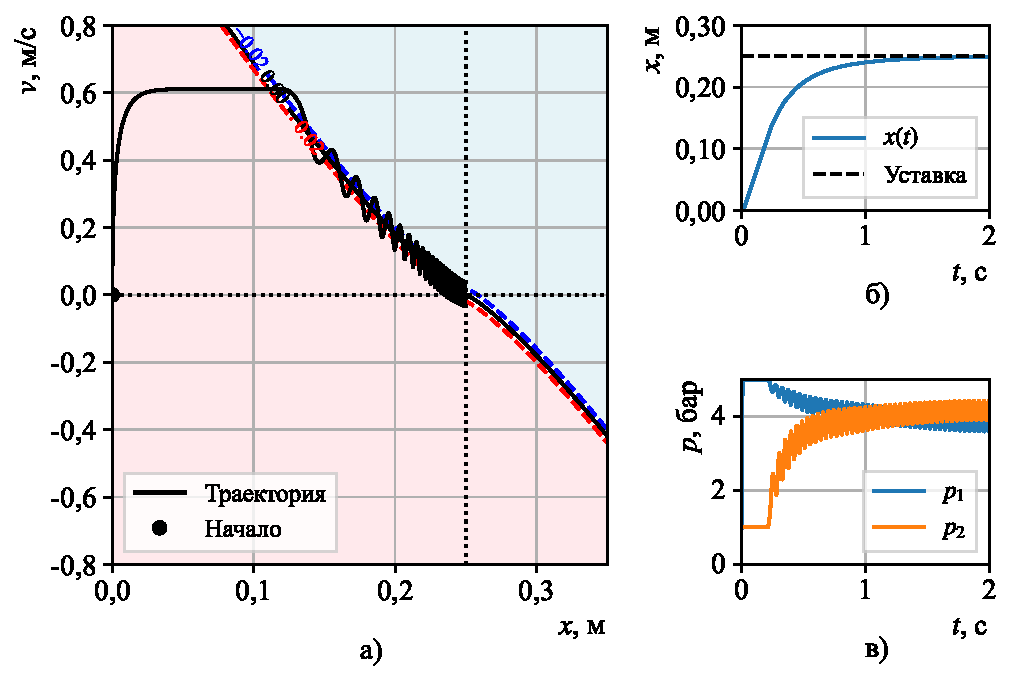
\includegraphics[]{part3/smc_teminal.pdf}
	\caption{Динамика системы с терминальной поверхностью скольжения
		при $p=9$, $q=11$ и $\beta=5$: а) фазовый портрет; б) переходной процесс; в) изменение давлений в полостях}
	\label{fig:smc_terminal}
\end{figure}


Анализ различных конфигураций многорежимного управления в скользящих режимах позволяет сделать следующие выводы:

\begin{enumerate}
	\item Трёхрежимное управление, хотя и обеспечивает достижение целевого положения, но имеет существенные
	      ограничения в точности позиционирования и стабильности процесса из-за компромисса между шириной $\varepsilon$-окрестности
	      поверхности скольжения и вероятностью возникновения «дребезга».

	\item Пятирежимное управление за счёт введения промежуточных режимов торможения позволяет существенно
	      улучшить характеристики процесса позиционирования, обеспечивая более плавное снижение
	      скорости и снижение статической ошибки без увеличения частоты переключений распределителей.

	\item Семирежимное управление обеспечивает наилучшие показатели качества позиционирования
	      среди рассмотренных конфигураций, создавая оптимальную градацию торможения перед достижением целевого положения.

	\item Интегральная поверхность скольжения обеспечивает нулевую статическую ошибку в
	      установившемся режиме и высокую робастность к постоянным возмущениям, что делает её предпочтительной для систем, работающих в условиях внешних нагрузок.

	\item Терминальная поверхность скольжения обеспечивает конечное время сходимости и
	      ускоренную сходимость при малых ошибках, что делает её предпочтительной для прецизионных систем с высокими требованиями к точности позиционирования.
\end{enumerate}

Выбор конкретной конфигурации (количество режимов и тип поверхности скольжения) должен осуществляться с учётом
требований к точности позиционирования, быстродействию и ресурсным показателям системы. Для этого в главе~\ref{ch:ch5} будет
представлена методика структурно-параметрического синтеза, позволяющая определить оптимальные параметры управления в зависимости от заданных критериев оптимизации.
\section{Использование нечеткой логики для управления пневмоприводом с дискретными распределителями}\label{sec:ch3/sec4}
\subsection*{Теоретические основы нечеткого управления пневмоприводом}\label{subsec:ch3/sec4/sub1}

Математический аппарат нечеткой логики для управления электропневматическим приводом
с дискретными распределителями основывается на формализации качественных экспертных знаний
о процессе управления с учетом специфики пневматических систем. Данный подход позволяет эффективно
преобразовывать лингвистические правила управления в конкретные управляющие воздействия на распределители.

В основе математического описания лежит определение нечеткого множества $A$ в
универсальном множестве $X$, характеризуемого
функцией принадлежности, как показано на рисунке \ref{fig:membership_functions}:
\begin{equation}
	\mu_A: X \rightarrow \left[0,1\right].
\end{equation}

\begin{figure}[ht]
	\centering
	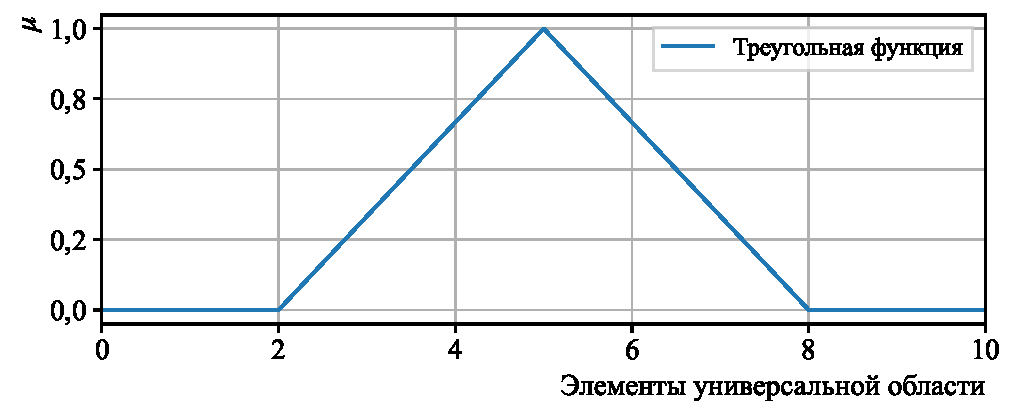
\includegraphics[]{part3/membership_function.pdf}
	\caption{Функция принадлежности нечеткого множества}
	\label{fig:membership_functions}
\end{figure}

Для формального описания процесса управления вводится понятие лингвистической переменной,
определяемой кортежем из пяти базовых элементов
\begin{equation}
	\langle \beta, T(\beta), X, G, M \rangle,
\end{equation}
где $\beta$ -- наименование лингвистической переменной;
$T(\beta)$ -- терм-множество значений, представляющее собой названия нечетких переменных;
$X$ -- универсальное множество, определяющее область значений рассматриваемой переменной;
$G$ -- синтаксические правила, порождающие названия значений лингвистической переменной;
$M$ -- семантические правила, задающие функции принадлежности нечетких термов.
\nomenclature{$\beta$}{Лингвистическая переменная\nomrefeqpage}
\nomenclature{$T(\beta)$}{Терм-множество значений\nomrefeqpage}
\nomenclature{$X$}{Универсальное множество\nomrefeqpage}
\nomenclature{$G$}{Синтаксические правила\nomrefeqpage}
\nomenclature{$M$}{Семантические правила\nomrefeqpage}


Для описания динамического состояния электропневматического привода
используются две основные лингвистические переменные:
\begin{equation}
	\beta = \left\{\beta_1, \beta_2\right\} = \left\{e, v\right\},
\end{equation}
где $e$ -- ошибка позиционирования;
$v$ -- скорость РО.

Дополнительно система может быть расширена путем включения информации о
давлениях в полостях пневмоцилиндра $p_1$ и $p_2$, что позволяет повысить
качество управления за счет учета термодинамических процессов.

Для ошибки позиционирования определяется следующая структура:
\begin{equation}
	\beta_1 = \text{<<ошибка позиционирования>>}
\end{equation}

\begin{equation}
	T(\beta_1) =\begin{cases}
		\text{Отрицательная большая}; \\
		\ldots                        \\
		\text{Нулевая}     ;          \\
		\ldots                        \\
		\text{Положительная большая},
	\end{cases}
\end{equation}
при

\begin{equation}
	X_1 = [-x_{\text{max}}, x_{\text{max}}],
\end{equation}
где $x_{\text{max}}$ -- максимально возможное отклонение от заданного положения.

Синтаксические правила $G$ в данном случае определяют способы формирования составных термов:
\begin{equation}
	\text{G}: \text{знак} + \text{размер},
\end{equation}
где <<знак>> $\in$ {Отрицательная, Положительная}; <<размер>> $\in$ {Малая, Средняя, Большая}

Семантические правила $M$ устанавливают соответствие между термами и их функциями принадлежности:
\begin{equation}
	M: T(\beta_1) \rightarrow {\mu_i(x) | x \in X_1}.
\end{equation}

Аналогично для скорости изменения ошибки:
\begin{equation}
	\beta_2 = \text{<<скорость>>}.
\end{equation}

\begin{equation}
	T(\beta_2) =\begin{cases}
		\text{Отрицательная большая}; \\
		\ldots                        \\
		\text{Нулевая} ;              \\
		\ldots                        \\
		\text{Положительная большая},
	\end{cases}
\end{equation}

\begin{equation}
	X_2 = [-v_{\text{max}}, v_{\text{max}}],
\end{equation}
где $v_{\text{max}}$ -- максимально допустимая скорость.

На рисунке \ref{fig:linguistic_variable_structure} представлена структура лингвистической переменной
<<ошибка позиционирования>> с
7 термами на универсальном множестве $X$ от $-0,2$ до $0,2$.

\begin{figure}[ht]
	\centering
	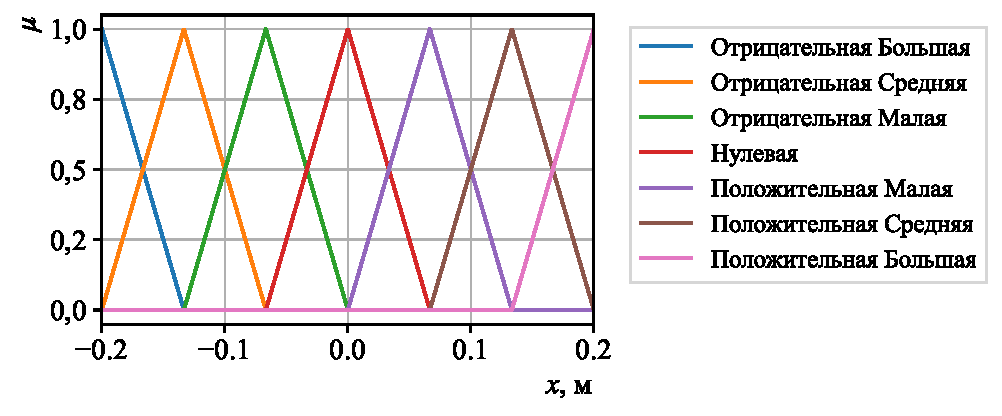
\includegraphics{part3/position_error_membership_functions.pdf}
	\caption{Структура лингвистической переменной}
	\label{fig:linguistic_variable_structure}
\end{figure}

Для каждого терма лингвистической переменной определяется функция принадлежности,
которая может быть представлена в различных формах,
как показано на рисунке \ref{fig:membership_functions_types}.
Наиболее распространенными являются:

Треугольная функция принадлежности:
\begin{equation}
	\mu_A(x; a, b, c) = \max\left(\min\left(\frac{x-a}{b-a}, \frac{c-x}{c-b}\right), 0\right).
\end{equation}

Гауссова функция принадлежности:
\begin{equation}\label{eq:gaussian_membership}
	\mu_A(x; c, \sigma) = \exp\left(-\frac{(x-c)^2}{2\sigma^2}\right).
\end{equation}

Z-образная функция принадлежности:
\begin{equation}\label{eq:z_membership}
	\mu_A(x; a, b) = \max\left(\min\left(\frac{x-a}{b-a}, 1\right), 0\right).
\end{equation}

Трапецеидальная функция принадлежности:
\begin{equation}
	\mu_A(x; a, b, c, d) = \max\left(\min\left(\frac{x-a}{b-a}, 1, \frac{d-x}{d-c}\right), 0\right).
\end{equation}

\begin{figure}[ht]
	\centering
	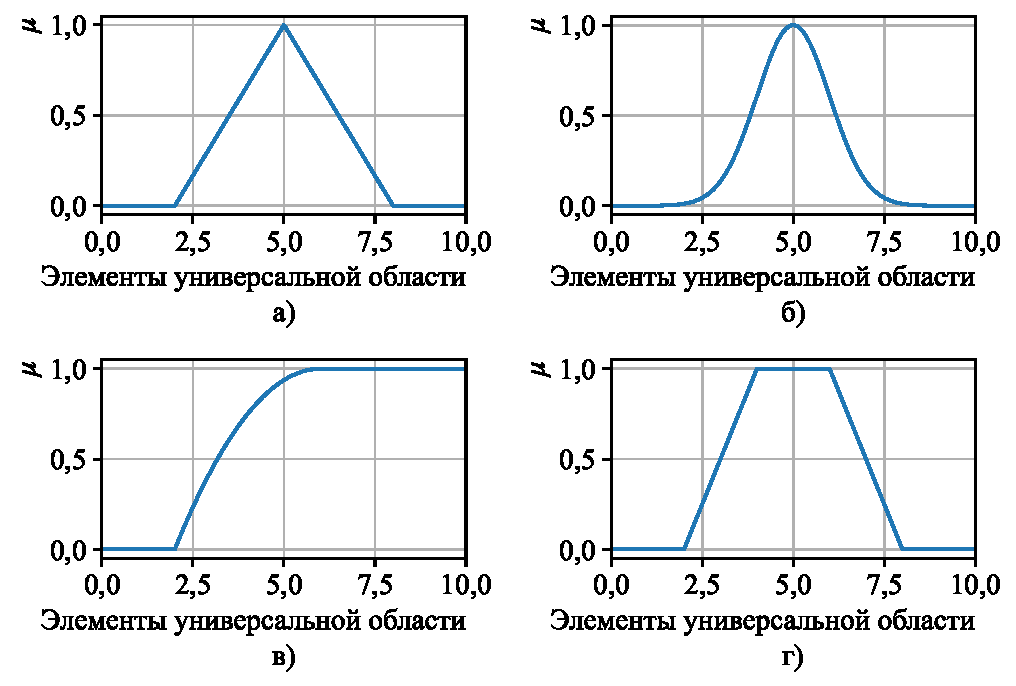
\includegraphics{part3/membership_functions.pdf}
	\caption{Типы функций принадлежности:\\
		а) треугольная; б) гауссова; в) z-образная; г) трапецеидальная}
	\label{fig:membership_functions_types}
\end{figure}

Важным аспектом определения лингвистической переменной является выбор
количества термов и их расположения
на универсальном множестве. При этом должны выполняться условия полноты:

\begin{equation}
	\forall x \in X: \sum_{i=1}^n \mu_i(x) > 0,
\end{equation}
и непротиворечивости:

\begin{equation}
	\forall x \in X: \sum_{i=1}^n \mu_i(x) \leq n,
\end{equation}
где $n$ -- количество термов.

База правил нечеткого вывода формируется на основе экспертных знаний
и представляется в виде продукционных правил согласно выражению \ref{eq:fuzzy_rule}. Такие правила как правило,
можно представить в табличном виде согласно рисунку \ref{fig:fuzzy_rules}:

\begin{equation}\label{eq:fuzzy_rule}
	R_i: \text{ЕСЛИ } e \text{ есть } A_i \text{ И } \dot{e} \text{ есть } B_i \text{ ТО } u \text{ есть } C_i.
\end{equation}

\begin{figure}[ht]
	\centering
	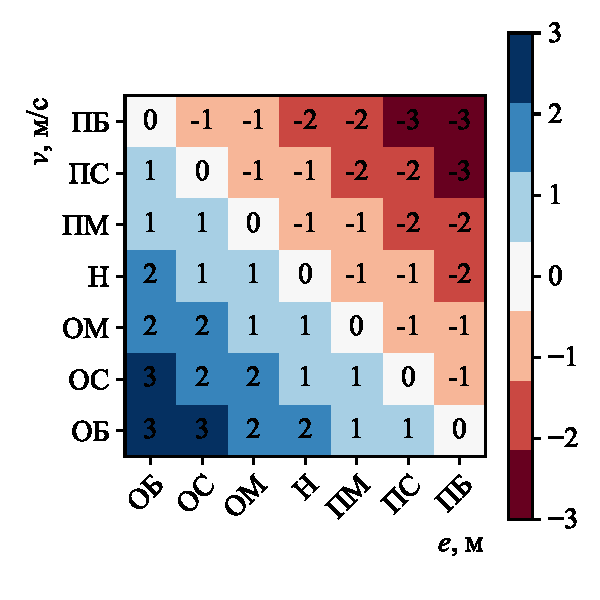
\includegraphics[]{part3/rule_base.pdf}
	\caption{Пример матрицы правил нечеткого вывода для электропневматического привода}
	\label{fig:fuzzy_rules}
\end{figure}

Процесс нечеткого логического вывода в разработанной системе управления реализуется в
соответствии с алгоритмом Мамдани, который включает последовательность
взаимосвязанных этапов преобразования информации, представленных на рисунке \ref{fig:fuzzy_inference}. Данный алгоритм
обеспечивает преобразование входных четких значений в выходные управляющие воздействия посредством
следующей математической процедуры.

На начальном этапе осуществляется фаззификация входных переменных, при которой определяется
степень принадлежности входных значений к различным нечетким множествам:
\begin{equation}
	\alpha_{ij} = \mu_{A_i}(e_j),
\end{equation}
где $\alpha_{ij}$ -- степень принадлежности входного значения $e_j$ к нечеткому множеству $A_i$;
$\mu_{A_i}(\cdot)$ - функция принадлежности соответствующего нечеткого множества.
\nomenclature{$\alpha_{ij}$}{Степень принадлежности входного значения $e_j$ к нечеткому множеству $A_i$\nomrefeqpage}
\nomenclature{$\mu_{A_i}(\cdot)$}{Функция принадлежности соответствующего нечеткого множества \nomrefeqpage}

Далее производится агрегирование подусловий в правилах нечеткого вывода путем
определения минимального значения степеней принадлежности:
\begin{equation}
	\alpha_i = \min(\alpha_{i1}, \alpha_{i2}),
\end{equation}
где $\alpha_i$ -- степень выполнения i-го правила нечеткой базы знаний.

На этапе активизации подзаключений формируются усеченные
функции принадлежности выходных лингвистических переменных:
\begin{equation}
	\mu'i(y) = \min(\alpha_i, \mu{C_i}(y)),
\end{equation}
где $\mu_{C_i}(y)$ -- функция принадлежности заключения i-го правила.

Аккумуляция заключений производится посредством объединения всех
усеченных функций принадлежности с использованием операции максимума:
\begin{equation}
	\mu_\Sigma(y) = \max_{i=1,m}\mu'_i(y).
\end{equation}

Заключительным этапом является дефаззификация результирующего
нечеткого множества, осуществляемая методом центра тяжести:
\begin{equation}
	y^* = \frac{\displaystyle\int\limits_{-\infty}^{+\infty} y\mu_\Sigma(y)dy}{\displaystyle\int\limits_{-\infty}^{+\infty} \mu_\Sigma(y)dy},
\end{equation}
где $y^*$ -- четкое значение выходной переменной, определяемое как центр тяжести площади под кривой
результирующей функции принадлежности $\mu_\Sigma(y)$.
\nomenclature{$y^*$}{Четкое значение выходной переменной, определяемое как центр тяжести площади под кривой результирующей функции принадлежности $\mu_\Sigma(y)$\nomrefeqpage}
В практической реализации пределы интегрирования ограничиваются областью определения
выходной переменной $[y_{min}, y_{max}]$, что обусловлено конечностью носителя нечеткого множества.

\begin{figure}[ht]
	\centering
	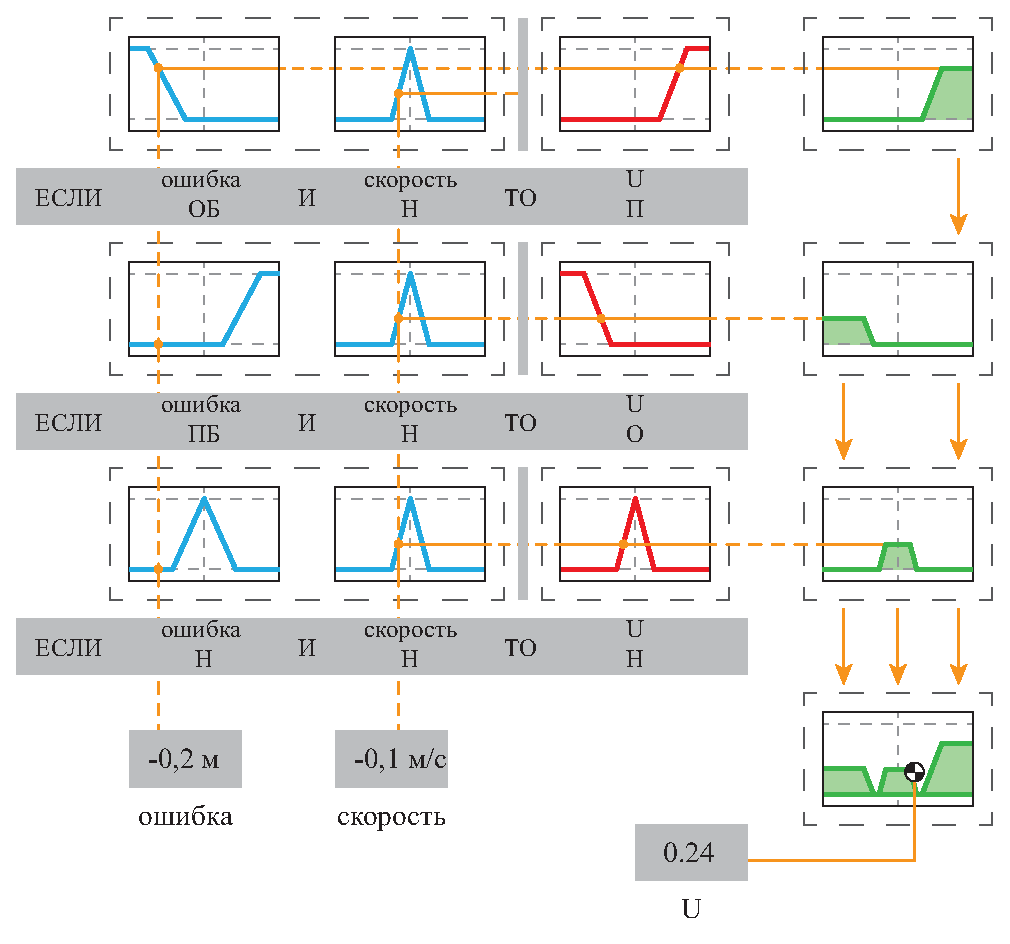
\includegraphics{part3/Мамдани.eps}
	\caption{Алгоритм Мамдани}
	\label{fig:fuzzy_inference}
\end{figure}

После выполнения дефаззификации осуществляется преобразование четкого значения управляющего воздействия
$y^*$ в дискретные режимы работы электропневматического привода посредством пороговой функции:
\begin{equation}
	\mathbf{u}(y^*) = \begin{cases}
		[1,0,0,1], & y^ \geq \varepsilon_2                   \\
		[1,0,0,0], & \varepsilon_1 < y^* \leq \varepsilon_2  \\
		[0,0,0,0], & |y^| \leq \varepsilon_1                 \\
		[0,0,1,0], & -\varepsilon_2 < y^ \leq -\varepsilon_1 \\
		[0,1,1,0], & y^* \leq -\varepsilon_2
	\end{cases}
\end{equation}
где $\varepsilon_1$, $\varepsilon_2$ ($\varepsilon_1 < \varepsilon_2$) -- пороговые значения, определяющие
границы переключения между режимами работы привода.
Данное преобразование обеспечивает формирование дискретных
управляющих воздействий на электромагнитные распределители в зависимости от
величины выходного сигнала нечеткого регулятора. При этом выбор
режима работы осуществляется таким образом, чтобы обеспечить плавное
изменение управляющего воздействия при переходе между различными состояниями системы.


\subsection*{Синтез нечеткого регулятора для пневмопривода с дискретными распределителями}\label{subsec:ch3/sec4/sub2}

Разработка матрицы правил нечеткой логики основывается на системном
анализе динамики пневмопривода. Процесс формирования базы правил можешь быть представлен
следующей последовательностью действий.
Первоначально определяются входные лингвистические переменные, как было показано в ранее, в данном случае это ошибка позиционирования и скорость:
\begin{enumerate}
	\item Ошибка позиционирования $e$;
	\item Скорость $v$.
\end{enumerate}

Далее происходит Фаззификация входных переменных с использованием следующих термов:
\begin{enumerate}
	\item Для ошибки: {ОБ (отрицательная большая),
	      ОМ (отрицательная малая),
	      Н (нулевая),
	      ПМ (положительная малая),
	      ПБ (положительная большая)};

	\item Для скорости: {ОБ (отрицательная большая),
	      ОМ (отрицательная малая),
	      Н (нулевая),
	      ПМ (положительная малая),
	      ПБ (положительная большая)};
\end{enumerate}

А так же определение функций принадлежности для каждого терма, согласно таблице
\ref{tab:operation_modes}:
\begin{enumerate}
	\item СиП (сильно положительная): [1,0,0,1];
	\item СрП (средне положительная): [1,0,0,0];
	\item СлП (слабо положительная): [0,0,0,1];
	\item Н: (нейтральная) [0,0,0,0];
	\item СлО (слабо отрицательная): [0,1,0,0];
	\item СрО (средне отрицательная): [0,0,1,0];
	\item СиО (сильно отрицательная): [0,1,1,0].
\end{enumerate}

В качестве функции принадлежности для крайних термов используется Z-образная функция \ref{eq:z_membership},
а для промежуточных термов применяется функция Гаусса \ref{eq:gaussian_membership}.

На рисунке \ref{fig:membership_functions_concrete} представлены функции принадлежности
для ошибки позиционирования и скорости соответственно.

\begin{figure}[ht]
	\centering
	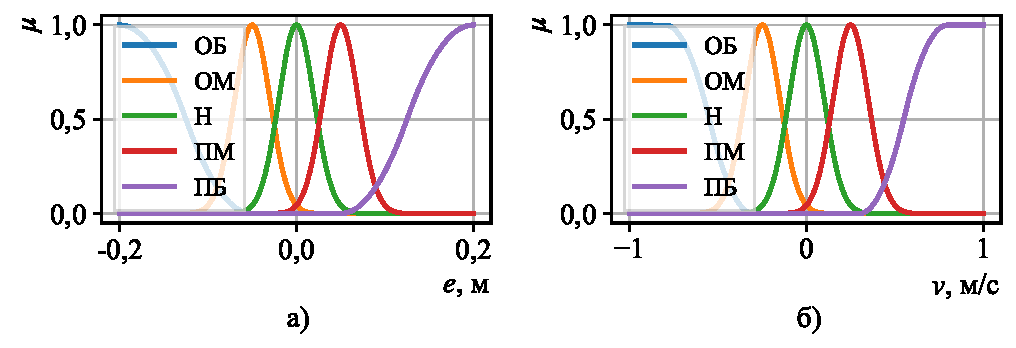
\includegraphics{part3/membership_functions_concrete.pdf}
	\caption{Функции принадлежности для ошибки позиционирования и скорости}
	\label{fig:membership_functions_concrete}
\end{figure}

Последним этапом происходит формирование базы правил нечеткого вывода, которая представляется
в виде матрицы, как показано на рисунке \ref{fig:fuzzy_rules}.

При разработке базы правил для нечеткого управления пневмоприводом
необходимо учитывать физические процессы, происходящие в системе.
Рассмотрим принцип формирования правил, основываясь на анализе
динамики пневмопривода.

При большой отрицательной ошибке, когда требуется движение влево,
учитываются различные физические состояния системы. В случае,
когда система уже движется влево с высокой скоростью, сохраняется
интенсивное управляющее воздействие, поскольку направление движения
соответствует требуемому. При замедлении движения влево применяется
умеренное воздействие для поддержания контролируемого движения.
Если система находится в состоянии покоя, осуществляется плавный
запуск движения для предотвращения резких динамических нагрузок.
В ситуации движения в неверном направлении (вправо) формируется
максимальное тормозящее усилие для изменения направления движения.

При малой отрицательной ошибке особое внимание уделяется
плавности движения. В случае быстрого движения влево начинается
постепенное торможение для предотвращения перерегулирования.
При медленном движении система переводится в режим удержания
позиции. Если наблюдается движение в неверном направлении,
формируется умеренное корректирующее воздействие.

В области нулевой ошибки основной задачей становится стабилизация
положения. При наличии остаточной скорости формируется тормозящее
усилие, пропорциональное скорости движения. В состоянии покоя все
распределители закрываются для минимизации расхода воздуха и
предотвращения автоколебаний.

Для малой положительной ошибки принципы формирования правил
аналогичны случаю малой отрицательной ошибки, но с противоположным
направлением воздействий. При большой положительной ошибке
логика управления зеркально отражает случай большой отрицательной ошибки.

Особое внимание при формировании правил уделяется учету сжимаемости
воздуха и существенного запаздывания между моментом переключения
распределителей и изменением давления в полостях цилиндра. Это
реализуется путем введения упреждающего торможения при высоких
скоростях движения. Также учитывается нелинейный характер изменения
давления в полостях цилиндра и влияние сил трения.

Каждое правило в базе формируется исходя из необходимости
обеспечения плавного движения с минимальным количеством
переключений распределителей при сохранении требуемого
быстродействия системы. При этом интенсивность управляющих
воздействий градуируется таким образом, чтобы обеспечить
оптимальное соотношение между скоростью реакции системы и
точностью позиционирования.

В результате получается база правил, представленная на рисунке \ref{fig:concrette_fuzzy_rules}, а результаты моделирования на \ref{fig:fuzzy_transient}.

\begin{figure}[ht]
	\centering
	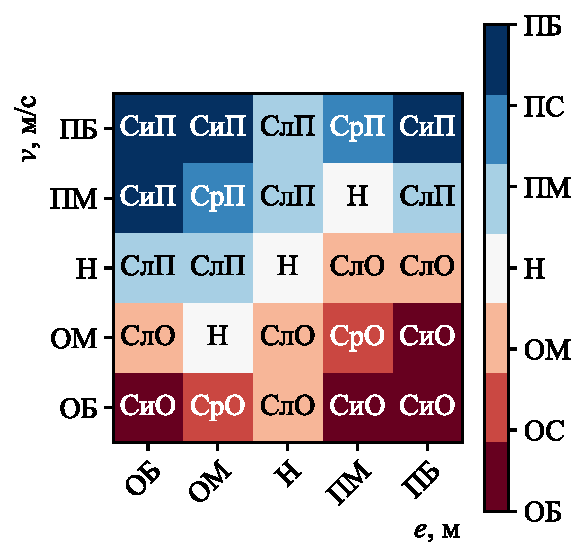
\includegraphics{part3/rule_base_concrete.pdf}
	\caption{База правил по конкретному описанию динамики пневмопривода}
	\label{fig:concrette_fuzzy_rules}
\end{figure}

\begin{figure}[ht]
	\centering
	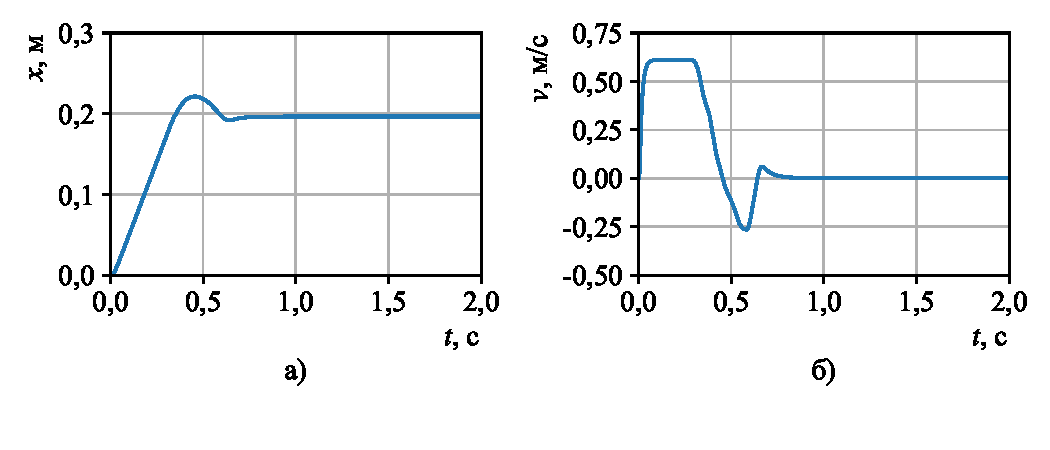
\includegraphics{part3/fuzzy_control.pdf}
	\caption{Переходной процесс для представленного нечетко-логического контроллера }
	\label{fig:fuzzy_transient}
\end{figure}

Важной особенностью разработанного нечеткого регулятора является адаптивное изменение интенсивности управляющего
воздействия в зависимости от текущего состояния системы, что позволяет минимизировать количество переключений распределителей при
сохранении удовлетворительного качества переходного процесса.

\section{Использование прогнозного управления}

\subsection*{Алгоритм прогнозного управления}

Прогнозное управление (Model Predictive Control, MPC) представляет собой один из наиболее
перспективных подходов к управлению нелинейными системами с ограничениями. В отличие от
традиционных методов управления, таких как ПИД-регулирование или управление в
скользящих режимах, прогнозное управление основано на решении задачи оптимизации
на каждом шаге управления с использованием математической модели объекта для прогнозирования его будущего поведения.

\paragraph*{Математическая формулировка прогнозного управления для пневмопривода.}

Принцип работы прогнозного управления заключается в использовании модели объекта для
прогнозирования его будущего поведения на определенном горизонте прогноза $N_p$ и определении
последовательности управляющих воздействий $\{u(k), u(k+1), ..., u(k+N_c-1)\}$ на горизонте управления
$N_c$ ($N_c \leq N_p$), минимизирующей заданную целевую функцию.
\nomenclature{$N_p$}{Горизонт прогноза\nomrefeqpage}
\nomenclature{$N_c$}{Горизонт управления\nomrefeqpage}

Для пневматического привода с дискретными распределителями задача прогнозного управления
формулируется следующим образом. В каждый момент времени $k$ известно текущее
состояние системы $x(k)$, включающее положение штока, скорость его движения и давления
в рабочих полостях. С использованием математической модели пневмопривода
выполняется прогноз состояний системы $\{x(k+1|k), x(k+2|k), ..., x(k+N_p|k)\}$ на
горизонте прогноза $N_p$ для различных последовательностей управляющих воздействий. На
основе полученных прогнозов выбирается такая последовательность управляющих
воздействий $\{u(k|k), u(k+1|k), ..., u(k+N_c-1|k)\}$, которая минимизирует целевую
функцию, учитывающую ошибку позиционирования, быстродействие системы и число переключений
распределителей. После чего применяется первое управляющее воздействие из
оптимальной последовательности $u(k) = u(k|k)$. На следующем шаге
управления $(k+1)$ процедура повторяется с учетом нового измеренного состояния системы $x(k+1)$.

Математическая модель электропневматического привода с дискретными распределителями в
упрощенном представлении описывается следующей системой дифференциальных уравнений:

\begin{equation}
	\begin{cases}
		\dot{x} = v;                                                                                                  \\
		\dot{v} = \frac{1}{M}(p_1 F_1 - p_2 F_2 - R_{\text{тр}}(v));                                                  \\
		\dot{p}_1 = \frac{\gamma R T}{V_1(x)}(\dot{m}_{\text{вх},1} - \dot{m}_{\text{вых},1} - \frac{p_1}{R T}F_1 v); \\
		\dot{p}_2 = \frac{\gamma R T}{V_2(x)}(\dot{m}_{\text{вх},2} - \dot{m}_{\text{вых},2} + \frac{p_2}{R T}F_2 v), \\
	\end{cases}
\end{equation}
где $x$ -- положение штока;
$v$ -- скорость штока;
$p_1$ и $p_2$ -- давления в поршневой и штоковой полостях соответственно;
$M$ -- масса подвижных частей;
$F_1$ и $F_2$ -- эффективные площади поршня
$R_{\text{тр}}(v)$ -- сила трения;
$\gamma$ -- показатель адиабаты;
$R$ -- газовая постоянная;
$T$ -- температура;
$V_1(x)$ и $V_2(x)$ -- объемы полостей;
$\dot{m}_{\text{вх},i}$ и $\dot{m}_{\text{вых},i}$ -- массовые расходы воздуха
через впускные и выпускные распределители для $i$-й полости.

Массовые расходы воздуха через распределители зависят от
их управляющих сигналов $u_i \in \{0, 1\}$ и могут быть описаны следующими выражениями:

\begin{equation}
	\begin{aligned}
		\dot{m}_{\text{вх},1}  & = u_1 \cdot C_1 \cdot f(p_\text{п}, p_1);    \\
		\dot{m}_{\text{вых},1} & = u_2 \cdot C_2 \cdot f(p_1, p_\text{атм});  \\
		\dot{m}_{\text{вх},2}  & = u_3 \cdot C_3 \cdot f(p_\text{п}, p_2);    \\
		\dot{m}_{\text{вых},2} & = u_4 \cdot C_4 \cdot f(p_2, p_\text{атм}) , \\
	\end{aligned}
\end{equation}
где $C_i$ -- проводимость $i$-го распределителя;
$p_\text{п}$ -- давление питания;
$p_\text{атм}$ -- атмосферное давление;
$f(p_u, p_d)$ -- функция, описывающая расход через распределитель
в зависимости от отношения давлений на входе $p_u$ и выходе $p_d$.

Для докритического режима течения ($p_d/p_u > b_{\text{кр}}$) аппроксимированная функция расхода имеет вид:

\begin{equation}
	f(p_u, p_d) = C_d F_\text{пр} \psi(r) p_u \sqrt{\frac{2}{RT}},
\end{equation}
где $r = p_d/p_u$ -- отношение давлений;
а $\psi(r)$ -- расходная функция, аппроксимированная полиномом:

\begin{equation}
	\psi(r) = 1 - a_1(1-r) - a_2(1-r)^2 - a_3(1-r)^3.
\end{equation}

Для критического режима ($p_d/p_u \leq b_{\text{кр}}$):

\begin{equation}
	f(p_u, p_d) = C_d F_\text{пр} \psi(b_{\text{кр}}) p_u \sqrt{\frac{2}{RT}},
\end{equation}
где $b_{\text{кр}} \approx \num{0.528}$ -- критическое отношение давлений для воздуха;

Особенностью прогнозного управления применительно к пневмоприводу с дискретными
распределителями является дискретный характер управляющих воздействий. В каждый момент времени
распределитель может находиться только в одном из двух состояний: открыт (1) или закрыт (0), что
существенно ограничивает пространство поиска оптимальных управляющих воздействий.
В то же время, за счет комбинации состояний четырех распределителей можно реализовать различные режимы работы привода.

В данной реализации используется 5-режимное управление, где каждый режим
соответствует определенной комбинации состояний распределителей:

\begin{enumerate}
	\item режим сильного положительного ускорения: $u = [1, 0, 0, 1]$;
	\item режим умеренного положительного ускорения: $u = [1, 0, 0, 0]$;
	\item режим удержания: $u = [0, 0, 0, 0]$;
	\item режим умеренного отрицательного ускорения: $u = [0, 0, 1, 0]$;
	\item режим сильного отрицательного ускорения: $u = [0, 1, 1, 0]$;
\end{enumerate}

\paragraph*{Целевая функция и алгоритм оптимизации.}

Для оценки качества управления используется целевая функция, минимизируемая на горизонте прогноза:

\begin{equation}
	\begin{aligned}
		J & = \sum_{i=1}^{N_p} Q_{\text{поз}} \cdot (x(k+i|k) - x_{\text{зад}})^2 +                 \\
		  & + \sum_{i=1}^{N_p} Q_{\text{скор}} \cdot v(k+i|k)^2 +                                   \\
		  & + \sum_{i=0}^{N_c-1} R_{\text{перекл}} \cdot \sum_{j=1}^{4} |u_j(k+i|k) - u_j(k+i-1|k)|,
	\end{aligned}
\end{equation}
где $Q_{\text{поз}}$ -- весовой коэффициент ошибки позиционирования;
$Q_{\text{скор}}$ -- весовой коэффициент скорости;
$R_{\text{перекл}}$ -- весовой коэффициент переключений распределителей;
$x_{\text{зад}}$ -- заданное положение.
\nomenclature{$Q_{\text{поз}}$}{Весовой коэффициент ошибки позиционирования\nomrefeqpage}
\nomenclature{$Q_{\text{скор}}$}{Весовой коэффициент скорости\nomrefeqpage}
\nomenclature{$R_{\text{перекл}}$}{Весовой коэффициент переключений распределителей\nomrefeqpage}

Первое слагаемое целевой функции отвечает за точность позиционирования,
второе -- за демпфирование колебаний (стремление к нулевой скорости в конце движения), третье -- за минимизацию числа переключений,
что способствует увеличению ресурса распределителей.

Классическая задача прогнозного управления требует решения на каждом шаге задачи оптимизации для
нахождения оптимальной последовательности управляющих воздействий. В случае дискретных распределителей
это задача комбинаторной оптимизации, полный перебор для которой требует значительных
вычислительных затрат. Для $N_c$ шагов управления и 5 возможных
режимов общее число вариантов составляет $5^{N_c}$, что становится
неприемлемым при увеличении горизонта управления.

Для сокращения вычислительной сложности в данной работе предложено использовать эвристический
подход, основанный на адаптивном формировании пространства поиска.
На основе текущего состояния системы (положения, скорости и ошибки позиционирования)
формируется ограниченное подмножество перспективных режимов управления для
первых нескольких шагов. Вместо полного перебора всех возможных последовательностей
длиной $N_c$ строится дерево решений с ограниченным фактором ветвления на каждом уровне. В
зависимости от величины и знака ошибки позиционирования, а также
текущей скорости, определяются предпочтительные режимы управления.
Например, при большой положительной ошибке $(e > \varepsilon_2)$ предпочтительны
режимы сильного и умеренного положительного ускорения; при малой ошибке
$(|e| \leq \varepsilon_1)$ предпочтителен режим удержания; при высокой скорости движения в
сторону, противоположную направлению к целевой точке, предпочтительны режимы торможения.

Алгоритм эвристического поиска оптимальной последовательности управляющих воздействий
может быть представлен следующим образом. На основе текущего состояния
системы $(x, v, p_1, p_2)$ и заданной точности позиционирования определяются
предпочтительные режимы управления для первого шага. Для каждого предпочтительного
режима первого шага прогнозируется состояние системы через один шаг по времени. На основе
прогнозируемого состояния определяются предпочтительные режимы для второго шага
и так далее до достижения заданной глубины поиска или горизонта управления.
Для каждой сформированной последовательности режимов прогнозируется траектория системы на
всем горизонте прогноза и вычисляется значение целевой функции. Затем выбирается
последовательность с минимальным значением целевой функции, и первый
режим из этой последовательности применяется в текущий момент времени.

Процесс генерации последовательностей управляющих воздействий можно описать
с использованием рекурсивного алгоритма. На каждом шаге алгоритм
принимает текущее состояние системы, текущую глубину рекурсии,
частичную последовательность режимов управления и список всех сгенерированных последовательностей.

Алгоритм продолжает работу до тех пор, пока не будет достигнута
максимальная глубина поиска. После этого сформированная последовательность
добавляется в общий список всех последовательностей. Такой подход позволяет
эффективно формировать множество возможных вариантов управления для
последующего анализа и выбора оптимального.

\paragraph*{Реализация алгоритма прогнозного управления.}

Для эффективной реализации алгоритма прогнозного управления пневмоприводом с дискретными
распределителями требуется
решить ряд практических задач. Полная термодинамическая модель пневмопривода слишком сложна
для использования в реальном времени, поэтому при работе алгоритма используется упрощенная модель,
обеспечивающая достаточную точность прогноза при значительно меньших вычислительных затратах.

Горизонт прогноза должен быть достаточно большим для адекватной оценки динамики системы,
но при этом не требовать чрезмерных вычислительных ресурсов. На основе экспериментальных исследований
установлено, что оптимальные значения горизонта прогноза находятся в диапазоне $8 \leq N_p \leq 15$.

Коэффициенты $Q_{\text{поз}}$, $Q_{\text{скор}}$ и $R_{\text{перекл}}$ определяют приоритеты
различных составляющих целевой функции и существенно влияют на поведение системы. Их подбор
осуществляется на основе анализа важности показателей качества.

Для работы в режиме реального времени необходимо оптимизировать алгоритм по быстродействию.
В данной работе это достигается за счет ограничения числа рассматриваемых последовательностей
управляющих воздействий, использования эвристик для отбора перспективных режимов,
адаптивного изменения шага моделирования в зависимости от динамики системы.

Для повышения устойчивости алгоритма к возмущениям и ошибкам модели реализованы защита
от численной нестабильности при моделировании, механизмы безопасного возврата к базовым
режимам управления при невозможности выполнения оптимизации и адаптация параметров в зависимости от текущей ошибки позиционирования.

На рисунке \ref{fig:mpc_transient} показан рассчитанный переходный процесс
пневмопривода с дискретными распределителями при использовании алгоритма прогнозного управления.

\begin{figure}[ht]
	\centering
	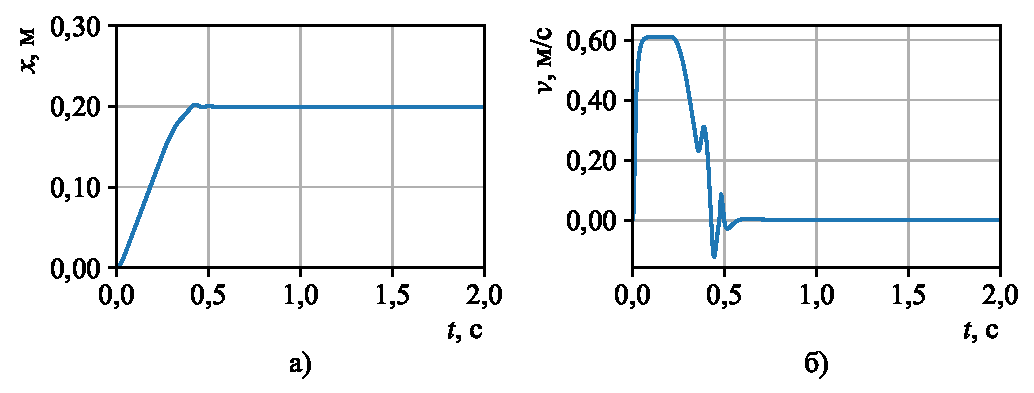
\includegraphics{part3/pneumatic_cylinder_mpc.pdf}
	\caption{Переходный процесс пневмопривода с дискретными распределителями при использовании алгоритма прогнозного управления}
	\label{fig:mpc_transient}
\end{figure}

Система прогнозного управления реализована как иерархическая структура,
включающая верхний уровень (формирование целевой траектории и параметров оптимизации),
средний уровень (решение задачи оптимизации и формирование последовательности управляющих режимов) и
нижний уровень (преобразование режимов в сигналы управления распределителями и их реализация).

Функционирование системы прогнозного управления может быть представлено
в виде блок-схемы, показанной на рисунке~\ref{fig:mpc_block_diagram}.

\begin{figure}[ht]
	\centering
	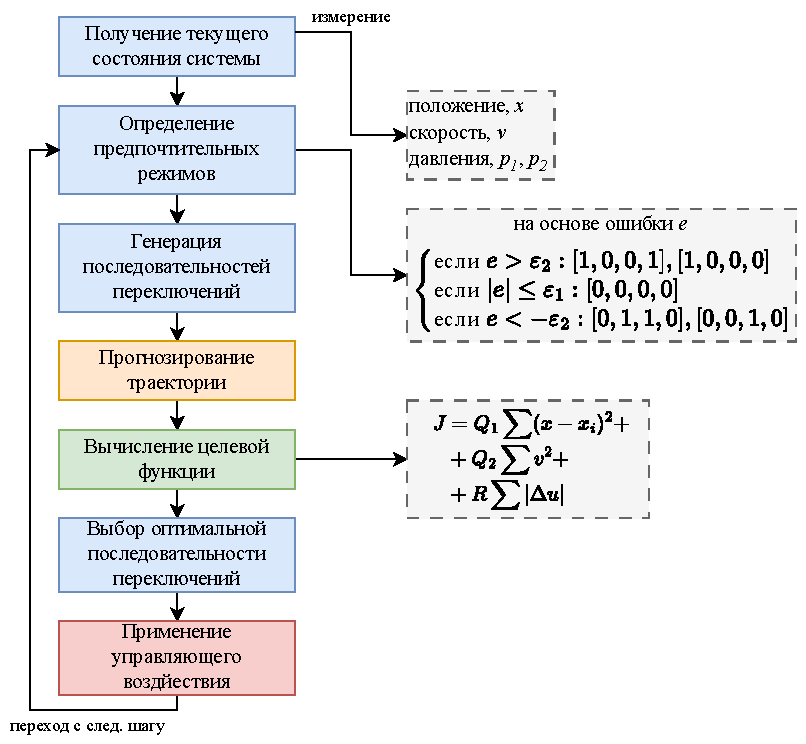
\includegraphics[width=\textwidth]{part3/mpc-block-diagram.pdf}
	\caption{Блок-схема системы прогнозного управления}
	\label{fig:mpc_block_diagram}
\end{figure}



\section{Выводы по главе 3}
На основе проведенного исследования методов управления электропневматическим приводом с дискретными распределителями можно сформулировать следующие основные выводы:

В результате теоретического анализа режимов работы электропневматического привода установлено, 
что динамика системы определяется сложным взаимодействием термодинамических и
механических процессов. Выявлено семь основных режимов функционирования, характеризующихся
различными комбинациями состояний распределителей, что позволяет осуществлять
гибкое управление движением рабочего органа.

Исследование модифицированного ПИД-регулятора с ШИМ показало возможность
существенного улучшения качества позиционирования за счет
введения адаптивного торможения на основе прогнозирования тормозного пути.
Предложенная модификация обеспечивает снижение устойчивый переходной процесс.

Разработанные алгоритмы управления в скользящих режимах с различными поверхностями
скольжения (линейной, интегральной и терминальной) демонстрируют
высокую робастность к параметрическим возмущениям.

Синтезированный нечеткий регулятор с пятью термами для входных переменных
обеспечивает плавное торможение и высокую точность позиционирования за счет
рациональной базы правил, учитывающей как ошибку, так и скорость её изменения.

Предложенные методы прогнозного управления, основанные на
упрощенной термодинамической модели привода, позволяют осуществлять
оптимизацию управляющих воздействий в реальном времени
с учетом ограничений на состояния системы и количество переключений распределителей.